
\renewcommand{\arraystretch}{1.8}
\footnotesize
\begin{longtable}[htp]
        {
            |>{\centering\hspace{0pt}}m{0.140\linewidth}
            |>{\hspace{0pt}}m{0.300\linewidth}
            |>{\centering\hspace{0pt}}m{0.140\linewidth}
            |>{\hspace{0pt}}m{0.300\linewidth}|
        } 
    \hline
    \multicolumn{4}{|c|}{{\cellcolor{maize}}{\Large\textbf{화 면 정 의 서}}} \\ 
    \hline
    시스템명 & TeulDa & 작성일 & 2021.01.10 \\ 
    \hline
    업 무 명 & 메인 화면 & 작성자 & 왕밤빵 \\ 
    \hline
    화면 ID & Main.jsp & 화면명 & Main \\ 
    \hline
    화면개요 & \multicolumn{3}{l|}{메인 화면} \\ 
    \hline
    \multicolumn{4}{|c|}{}\\
    \multicolumn{4}{|l|}{\textbf{1. 화면 레이아웃}} \\ 
    \multicolumn{4}{|c|}{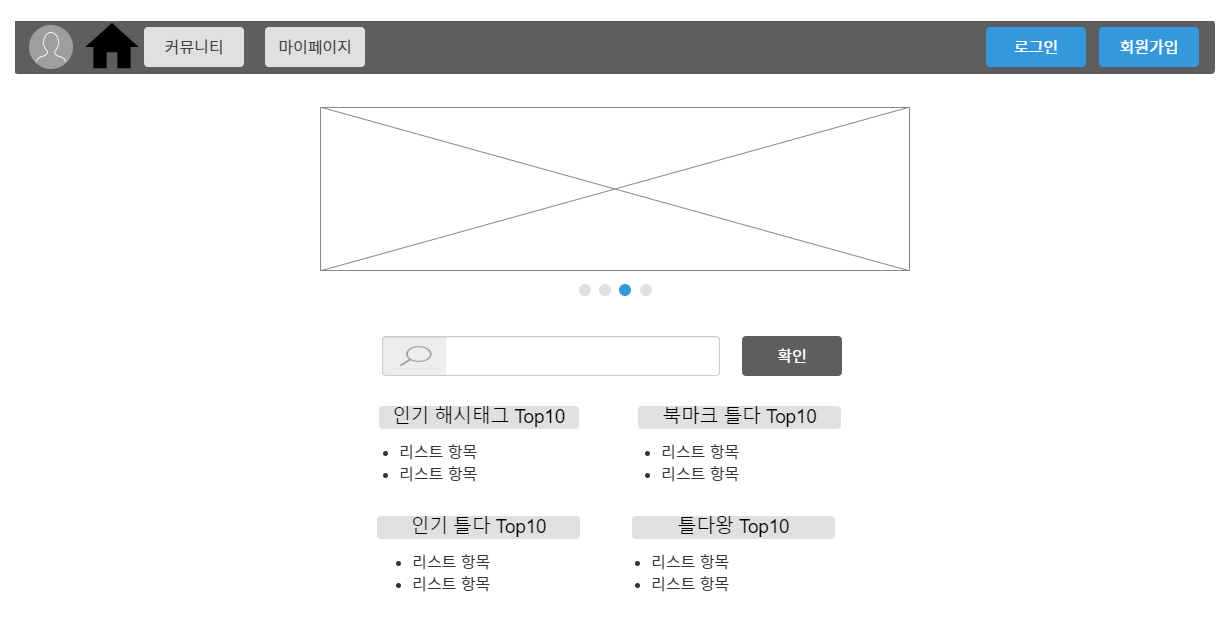
\includegraphics[width=17.00cm]{./Figure/Analysis/Display/main.png}} \\
    \hline
\end{longtable}

\textbf{2. 데이터 구성 항목}

\begin{longtable}
    {
        |>{\centering\hspace{0pt}}m{0.150\linewidth}
        |>{\centering\hspace{0pt}}m{0.180\linewidth}
        |>{\centering\hspace{0pt}}m{0.060\linewidth}
        |>{\centering\hspace{0pt}}m{0.110\linewidth}
        |>{\hspace{0pt}}m{0.150\linewidth}
        |>{\arraybackslash\hspace{0pt}}m{0.190\linewidth}|
    } 
    \hline
    \rowcolor{maize} 항목명(한글) & 컨트롤(영문) & 필수 & 수정여부 & \centering{설명} & \centering{비고/제약사항} \endhead 
    \hline
    검색어 & searchKeyword & Y & Y & 검색어 입력
    & \multicolumn{1}{>{\hspace{0pt}}m{0.190\linewidth}|}{} \\
    \hline
\end{longtable}

\textbf{3. 처리 로직}

\arrayrulecolor{black}
\begin{longtable}
    {
        |>{\hspace{0pt}}m{0.145\linewidth}
        |>{\hspace{0pt}}m{0.140\linewidth}
        |>{\hspace{0pt}}m{0.300\linewidth}
        |>{\hspace{0pt}}m{0.140\linewidth}
        |>{\hspace{0pt}}m{0.140\linewidth}|} 
    \hline
    \rowcolor{maize} 
    \multicolumn{1}{
        |>{\centering\hspace{0pt}}m{0.145\linewidth}|}{{\cellcolor{maize}}} 
        & \multicolumn{1}{>{\centering\hspace{0pt}}m{0.140\linewidth}|}{입력값/파라미터} 
        & \multicolumn{1}{>{\centering\hspace{0pt}}m{0.300\linewidth}|}{처리내용} 
        & \multicolumn{1}{>{\centering\hspace{0pt}}m{0.140\linewidth}|}{출력/처리결과} 
        & \multicolumn{1}{>{\centering\arraybackslash\hspace{0pt}}m{0.140\linewidth}|}{{\cellcolor{maize}}} \\* 
    \hhline{|>{\arrayrulecolor{maize}}->{\arrayrulecolor{black}}|--->{\arrayrulecolor{maize}}->{\arrayrulecolor{black}}|}
    \rowcolor{maize} 
        \multicolumn{1}{|>{\Centering\hspace{0pt}}m{0.145\linewidth}|}{\multirow{-2}{=}{\cellcolor{maize}\Centering{}이벤트명}} 
        & \multicolumn{1}{>{\Centering\hspace{0pt}}m{0.140\linewidth}|}{시작 JSP} 
        & \multicolumn{1}{>{\Centering\hspace{0pt}}m{0.300\linewidth}|}{프리젠테이션 레이어 설계} 
        & \multicolumn{1}{>{\Centering\hspace{0pt}}m{0.140\linewidth}|}{출력 JSP} 
        & \multicolumn{1}{>{\Centering\hspace{0pt}}m{0.140\linewidth}|}{\multirow{-2}{=}{\cellcolor{maize}\Centering{}비고}} \endhead
    \hline
    \multirow{4}{=}{확인.onClick()} & 검색어 & \multirow{2}{=}{입력값으로 검색한 결과 화면을 보여준다.} & 검색 결과 화면 이동 &  \\* 
     \arrayrulecolor[rgb]{0.8,0.8,0.8}\cline{2-2}\arrayrulecolor[rgb]{0.8,0.8,0.8}\cline{4-4}
     &  &  &  &  \\* 
    \arrayrulecolor{black}\cline{2-5}
     & \multicolumn{1}{>{\hspace{0pt}}m{0.140\linewidth}|}{Main.jsp} & \multicolumn{1}{>{\hspace{0pt}}m{0.300\linewidth}|}{Path : /community/getAll : GET} & totalSearch.jsp &  \\* 
     \arrayrulecolor[rgb]{0.8,0.8,0.8}\cline{2-2}\arrayrulecolor{black}\cline{3-3}\arrayrulecolor[rgb]{0.8,0.8,0.8}\cline{4-4}\arrayrulecolor{black}
     &  & \multicolumn{1}{>{\hspace{0pt}}m{0.300\linewidth}|}{Controller : com.teulda.web.community. communityController.getAll()} &  &  \\* 
    %  &  & {Controller : com.teulda.web.community.communityController.getAll()} &  &  \\ 
    \arrayrulecolor{black}\hline

    \multirow{4}{=}{인기 해시태그 Top10 리스트 항목 중 한개.onClick()} & 검색어(해시태그) & \multirow{2}{=}{입력값(해시태그)으로 검색한 화면을 보여준다.} & 검색 결과 화면 이동 &  \\* 
     \arrayrulecolor[rgb]{0.8,0.8,0.8}\cline{2-2}\arrayrulecolor[rgb]{0.8,0.8,0.8}\cline{4-4}
     &  &  &  &  \\* 
    \arrayrulecolor{black}\cline{2-5}
     & \multicolumn{1}{>{\hspace{0pt}}m{0.140\linewidth}|}{Main.jsp} & \multicolumn{1}{>{\hspace{0pt}}m{0.300\linewidth}|}{Path : /community/getAll : GET} & totalSearch.jsp &  \\* 
     \arrayrulecolor[rgb]{0.8,0.8,0.8}\cline{2-2}\arrayrulecolor{black}\cline{3-3}\arrayrulecolor[rgb]{0.8,0.8,0.8}\cline{4-4}\arrayrulecolor{black}
     &  & Controller : com.teulda.web.community. communityController.getAll() &  &  \\ 
    \arrayrulecolor{black}\hline

    \multirow{4}{=}{북마크 틀다 Top10 리스트 항목 중 한개.onClick()} & 기록번호 & \multirow{2}{=}{기록번호와 일치하는 기록 상세조회 화면을 보여준다.} & 기록 상세조회 화면 이동 &  \\* 
     \arrayrulecolor[rgb]{0.8,0.8,0.8}\cline{2-2}\arrayrulecolor[rgb]{0.8,0.8,0.8}\cline{4-4}
     &  &  &  &  \\* 
    \arrayrulecolor{black}\cline{2-5}
     & \multicolumn{1}{>{\hspace{0pt}}m{0.140\linewidth}|}{Main.jsp} & \multicolumn{1}{>{\hspace{0pt}}m{0.300\linewidth}|}{Path : /diary/getDiary} & getDiary.jsp &  \\* 
     \arrayrulecolor[rgb]{0.8,0.8,0.8}\cline{2-2}\arrayrulecolor{black}\cline{3-3}\arrayrulecolor[rgb]{0.8,0.8,0.8}\cline{4-4}\arrayrulecolor{black}
     &  & Controller : com.TeulDa.web.diary.DiaryC ontroller.getDiary() &  &  \\ 
    \arrayrulecolor{black}\hline

    \multirow{4}{=}{인기 틀다 Top10 리스트 항목 중 한개.onClick()} & 기록번호 & \multirow{2}{=}{기록번호와 일치하는 기록 상세조회 화면을 보여준다.} & 기록 상세조회 화면 이동 &  \\* 
     \arrayrulecolor[rgb]{0.8,0.8,0.8}\cline{2-2}\arrayrulecolor[rgb]{0.8,0.8,0.8}\cline{4-4}
     &  &  &  &  \\* 
    \arrayrulecolor{black}\cline{2-5}
     & \multicolumn{1}{>{\hspace{0pt}}m{0.140\linewidth}|}{Main.jsp} & \multicolumn{1}{>{\hspace{0pt}}m{0.300\linewidth}|}{Path : /diary/getDiary} & getDiary.jsp &  \\* 
     \arrayrulecolor[rgb]{0.8,0.8,0.8}\cline{2-2}\arrayrulecolor{black}\cline{3-3}\arrayrulecolor[rgb]{0.8,0.8,0.8}\cline{4-4}\arrayrulecolor{black}
     &  & Controller : com.TeulDa.web.diary.DiaryC ontroller.getDiary() &  &  \\ 
    \arrayrulecolor{black}\hline

    \multirow{4}{=}{틀다왕 Top10 리스트 항목 중 한개.onClick()} & 닉네임 & \multirow{2}{=}{닉네임과 일치하는 회원 프로필 화면을 보여준다.} & 회원 프로필 화면 이동 &  \\* 
     \arrayrulecolor[rgb]{0.8,0.8,0.8}\cline{2-2}\arrayrulecolor[rgb]{0.8,0.8,0.8}\cline{4-4}
     &  &  &  &  \\* 
    \arrayrulecolor{black}\cline{2-5}
     & \multicolumn{1}{>{\hspace{0pt}}m{0.140\linewidth}|}{Main.jsp} & \multicolumn{1}{>{\hspace{0pt}}m{0.300\linewidth}|}{Path :  /user/getUser : GET} & getUser.jsp &  \\* 
     \arrayrulecolor[rgb]{0.8,0.8,0.8}\cline{2-2}\arrayrulecolor{black}\cline{3-3}\arrayrulecolor[rgb]{0.8,0.8,0.8}\cline{4-4}\arrayrulecolor{black}
     &  & Controller : com.TeulDa.web.user.UserCon troller.getU ser() &  &  \\ 
    \arrayrulecolor{black}\hline
\end{longtable}
\clearpage
\newpage

\footnotesize
\begin{longtable}[htp]
        {
            |>{\centering\hspace{0pt}}m{0.140\linewidth}
            |>{\hspace{0pt}}m{0.300\linewidth}
            |>{\centering\hspace{0pt}}m{0.140\linewidth}
            |>{\hspace{0pt}}m{0.300\linewidth}|
        } 
    \hline
    \multicolumn{4}{|c|}{{\cellcolor{maize}}{\Large\textbf{화 면 정 의 서}}} \\ 
    \hline
    시스템명 & TeulDa & 작성일 & 2021.01.02 \\ 
    \hline
    업 무 명 & 회원관리 & 작성자 & 김채경 \\ 
    \hline
    화면 ID & addUser & 화면명 & 회원가입 \\ 
    \hline
    화면개요 & \multicolumn{3}{l|}{회원가입 화면} \\ 
    \hline
    \multicolumn{4}{|c|}{}\\
    \multicolumn{4}{|l|}{\textbf{1. 화면 레이아웃}} \\ 
    \multicolumn{4}{|l|}{\hspace{6pt}{자사회원 가입시}} \\ 
    \multicolumn{4}{|c|}{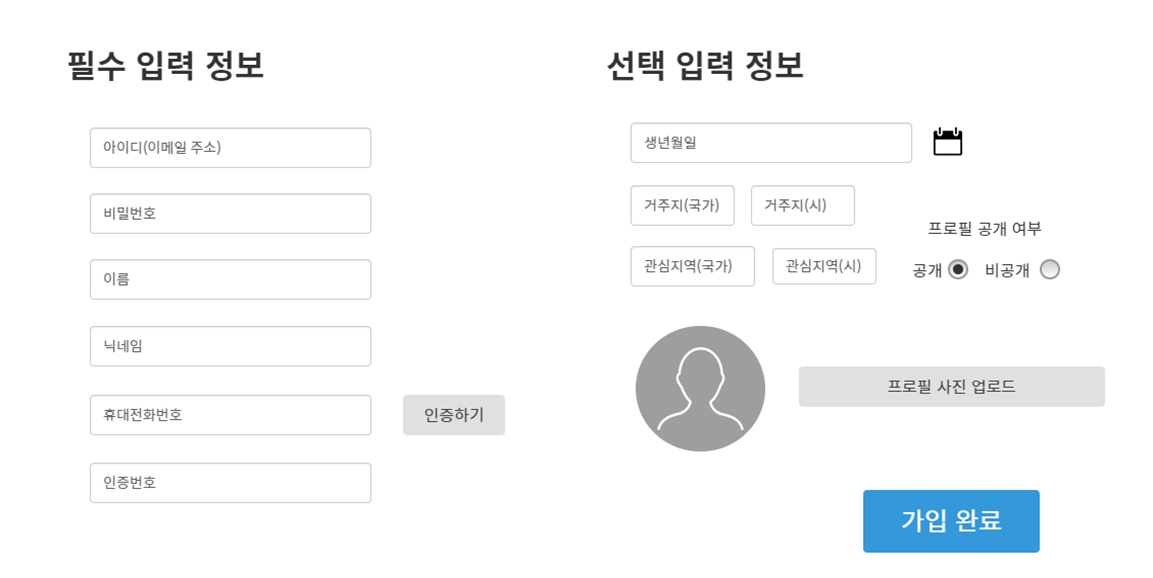
\includegraphics[width=17.00cm]{./Figure/Analysis/Display/addusert.png}} \\

    \multicolumn{4}{|l|}{\hspace{6pt}{소셜회원 가입시}} \\ 
    \multicolumn{4}{|c|}{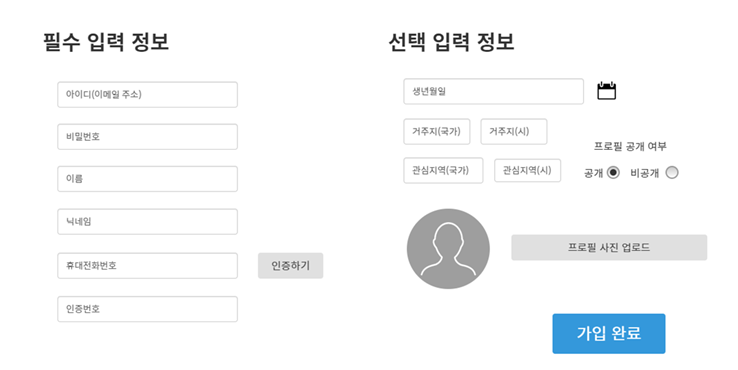
\includegraphics[width=17.00cm]{./Figure/Analysis/Display/addusers.png}} \\

    \hline
\end{longtable}

\par\
\par\
\textbf{2. 데이터 구성 항목}

\begin{longtable}
    {
        |>{\centering\hspace{0pt}}m{0.150\linewidth}
        |>{\centering\hspace{0pt}}m{0.180\linewidth}
        |>{\centering\hspace{0pt}}m{0.060\linewidth}
        |>{\centering\hspace{0pt}}m{0.110\linewidth}
        |>{\hspace{0pt}}m{0.150\linewidth}
        |>{\arraybackslash\hspace{0pt}}m{0.190\linewidth}|
    } 
    \hline
    \rowcolor{maize} 항목명(한글) & 컨트롤(영문) & 필수 & 수정여부 & \centering{설명} & \centering{비고/제약사항} \endhead 
    \hline
    아이디 & userId & Y & N & 사용자 아이디(이메일) 입력 & 소셜 로그인 시 입력 불가 \\ 
    \hline
    비밀번호 & password & Y & Y & 사용자 비밀번호 입력 & 6자 이상 입력, 소셜 로그인 시 입력 불가 \\ 
    \hline
    이름 & userName & Y & Y & 사용자 이름 입력 & 특수문자 사용 불가 \\ 
    \hline
    닉네임 & userNick & Y & N & 사용자 닉네임 입력 & 특수문자 사용 불가 \\ 
    \hline
    휴대전화번호 & userPhone & Y & Y & 사용자 휴대전화번호 입력 & 숫자만 입력 가능 \\ 
    \hline
    생년월일 & birthday & Y & Y & 사용자 생년월일 입력 &  \\ 
    \hline
    거주지 & resi & Y & Y & 사용자 거주지 입력 & 국가-시 \\ 
    \hline
    관심 여행지역 & interest & Y & Y & 사용자 관심지역 입력 & 국가-시 \\ 
    \hline
    프로필 사진 & myPhoto & Y & Y & 사용자 프로필사진 업로드 & 1장 \\ 
    \hline
    프로필 공개 여부 & openPro & N & Y & 해당 계정을 다른 사용자에 공개 할 지 여부 결정 & 공개 : 0 / 비공개 : 1 \\ 
    \hline
    인증번호 & conNumber & Y & Y & 회원가입 시 본인 핸드폰번호 인증~ & 번호 하나당 한 계정만 생성가능, 세션시간 5분 제공 \\ 
    \hline
    계정 상태 & status & Y & N & 활성화, 정지, 휴면 세가지 상태로 구분 & Hidden,계정 생성시 `활성화' default 활성화 : 0 / 정지 : 1 / 휴면 : 2 \\ 
    \hline
    계정 상태 변경일 & statusDate & Y & N & 계정 상태가 정지, 혹은 휴면상태로 바뀌었을 때 각 상태에 따른 조치 자동화를 위한 데이터 & Hidden, 정지 상태에서 2주 경과시 자동 활성화 휴면상태에서 1달 이내로 접속 시 자동 활성화, 그렇지 않을 경우 데이터 삭제 (년도-월-일) \\ 
    \hline
    역할 & role & Y & Y & 사용자의 계정 역할 구분 & Hidden, 사용자와 관리자 구분 회원 : user / 관리자 : admin \\
    \hline
\end{longtable}

\textbf{3. 처리 로직}

\arrayrulecolor{black}
\begin{longtable}
    {
        |>{\hspace{0pt}}m{0.145\linewidth}
        |>{\hspace{0pt}}m{0.140\linewidth}
        |>{\hspace{0pt}}m{0.300\linewidth}
        |>{\hspace{0pt}}m{0.140\linewidth}
        |>{\hspace{0pt}}m{0.140\linewidth}|} 
    \hline
    \rowcolor{maize} 
    \multicolumn{1}{
        |>{\centering\hspace{0pt}}m{0.145\linewidth}|}{{\cellcolor{maize}}} 
        & \multicolumn{1}{>{\centering\hspace{0pt}}m{0.140\linewidth}|}{입력값/파라미터} 
        & \multicolumn{1}{>{\centering\hspace{0pt}}m{0.300\linewidth}|}{처리내용} 
        & \multicolumn{1}{>{\centering\hspace{0pt}}m{0.140\linewidth}|}{출력/처리결과} 
        & \multicolumn{1}{>{\centering\arraybackslash\hspace{0pt}}m{0.140\linewidth}|}{{\cellcolor{maize}}} \\* 
    \hhline{|>{\arrayrulecolor{maize}}->{\arrayrulecolor{black}}|--->{\arrayrulecolor{maize}}->{\arrayrulecolor{black}}|}
    \rowcolor{maize} 
        \multicolumn{1}{|>{\Centering\hspace{0pt}}m{0.145\linewidth}|}{\multirow{-2}{=}{\cellcolor{maize}\Centering{}이벤트명}} 
        & \multicolumn{1}{>{\Centering\hspace{0pt}}m{0.140\linewidth}|}{시작 JSP} 
        & \multicolumn{1}{>{\Centering\hspace{0pt}}m{0.300\linewidth}|}{프리젠테이션 레이어 설계} 
        & \multicolumn{1}{>{\Centering\hspace{0pt}}m{0.140\linewidth}|}{출력 JSP} 
        & \multicolumn{1}{>{\Centering\hspace{0pt}}m{0.140\linewidth}|}{\multirow{-2}{=}{\cellcolor{maize}\Centering{}비고}} \endhead
    \hline
    \multirow{4}{=}{Client요청시(onLoad()시)} &  & \multirow{2}{=}{} &  &  \\* 
     \arrayrulecolor[rgb]{0.8,0.8,0.8}\cline{2-2}\arrayrulecolor[rgb]{0.8,0.8,0.8}\cline{4-4}
     &  &  &  &  \\* 
    \arrayrulecolor{black}\cline{2-5}
     & \multicolumn{1}{>{\hspace{0pt}}m{0.140\linewidth}|}{회원가입 UI} & \multicolumn{1}{>{\hspace{0pt}}m{0.300\linewidth}|}{Path : URI} & 회원가입 UI &  \\* 
     \arrayrulecolor[rgb]{0.8,0.8,0.8}\cline{2-2}\arrayrulecolor{black}\cline{3-3}\arrayrulecolor[rgb]{0.8,0.8,0.8}\cline{4-4}\arrayrulecolor{black}
     &  & \multicolumn{1}{>{\hspace{0pt}}m{0.300\linewidth}|}{Controller : 회원관리Ctrl} &  &  \\* 
    %  &  & {Controller : com.teulda.web.community.communityController.getAll()} &  &  \\ 
    \arrayrulecolor{black}\hline

    \multirow{4}{=}{인증하기.onClick()} & 전화번호 & \multirow{2}{=}{미리 입력한 전화번호로 인증번호문자 전송 및 팝업창으로 인증문자전송 안내} &  &  \\* 
     \arrayrulecolor[rgb]{0.8,0.8,0.8}\cline{2-2}\arrayrulecolor[rgb]{0.8,0.8,0.8}\cline{4-4}
     &  &  &  &  \\* 
    \arrayrulecolor{black}\cline{2-5}
     & \multicolumn{1}{>{\hspace{0pt}}m{0.140\linewidth}|}{회원가입 UI} & \multicolumn{1}{>{\hspace{0pt}}m{0.300\linewidth}|}{Path : URI } &  &  \\* 
     \arrayrulecolor[rgb]{0.8,0.8,0.8}\cline{2-2}\arrayrulecolor{black}\cline{3-3}\arrayrulecolor[rgb]{0.8,0.8,0.8}\cline{4-4}\arrayrulecolor{black}
     &  & Controller : 회원관리Ctrl & 회원가입 UI &  \\ 
    \arrayrulecolor{black}\hline

    \multirow{4}{=}{프로필 사진 업로드.onClick()} & 사진 파일 & \multirow{2}{=}{프로필 사진 업로드 팝업창 출력} &  &  \\* 
     \arrayrulecolor[rgb]{0.8,0.8,0.8}\cline{2-2}\arrayrulecolor[rgb]{0.8,0.8,0.8}\cline{4-4}
     &  &  &  &  \\* 
    \arrayrulecolor{black}\cline{2-5}
     & \multicolumn{1}{>{\hspace{0pt}}m{0.140\linewidth}|}{회원가입 UI} & \multicolumn{1}{>{\hspace{0pt}}m{0.300\linewidth}|}{Path : URI} &  &  \\* 
     \arrayrulecolor[rgb]{0.8,0.8,0.8}\cline{2-2}\arrayrulecolor{black}\cline{3-3}\arrayrulecolor[rgb]{0.8,0.8,0.8}\cline{4-4}\arrayrulecolor{black}
     &  & Controller : 회원관리Ctrl &  &  \\ 
    \arrayrulecolor{black}\hline

    \multirow{4}{=}{가입완료.onClick()} & e-mail, 비밀번호, 닉네임, 이름, 핸드폰 번호, 거주지(국가, 도시), 관심 여행지역(국가, 도시), 생년월일, 프로필사진(1개) & \multirow{2}{=}{회원가입완료화면으로 Navigation 및 입력정보 DB저장} & 이메일 인증화면으로 이동 & \multirow{4}{=}{필수 입력 사항을 입력하지 않거나 인증번호가 틀렸을 경우 재입력 요구 팝업창 출력} \\* 
     \arrayrulecolor[rgb]{0.8,0.8,0.8}\cline{2-2}\arrayrulecolor[rgb]{0.8,0.8,0.8}\cline{4-4}
     &  &  &  &  \\* 
    \arrayrulecolor{black}\cline{2-4}
     & \multicolumn{1}{>{\hspace{0pt}}m{0.140\linewidth}|}{회원가입 UI} & \multicolumn{1}{>{\hspace{0pt}}m{0.300\linewidth}|}{Path : URI} &  &  \\* 
     \arrayrulecolor[rgb]{0.8,0.8,0.8}\cline{2-2}\arrayrulecolor{black}\cline{3-3}\arrayrulecolor[rgb]{0.8,0.8,0.8}\cline{4-4}\arrayrulecolor{black}
     &  & Controller : 회원관리Ctrl & 이메일 인증 UI &  \\ 
    \arrayrulecolor{black}\hline

\end{longtable}
\newpage

\footnotesize
\begin{longtable}[htp]
        {
            |>{\centering\hspace{0pt}}m{0.140\linewidth}
            |>{\hspace{0pt}}m{0.300\linewidth}
            |>{\centering\hspace{0pt}}m{0.140\linewidth}
            |>{\hspace{0pt}}m{0.300\linewidth}|
        } 
    \hline
    \multicolumn{4}{|c|}{{\cellcolor{maize}}{\Large\textbf{화 면 정 의 서}}} \\ 
    \hline
    시스템명 & TeulDa & 작성일 & 2021.01.02 \\ 
    \hline
    업 무 명 & 회원관리 & 작성자 & 김채경 \\ 
    \hline
    화면 ID & login & 화면명 & 로그인 \\ 
    \hline
    화면개요 & \multicolumn{3}{l|}{로그인 화면} \\ 
    \hline
    \multicolumn{4}{|c|}{}\\
    \multicolumn{4}{|l|}{\textbf{1. 화면 레이아웃}} \\ 
    \multicolumn{4}{|c|}{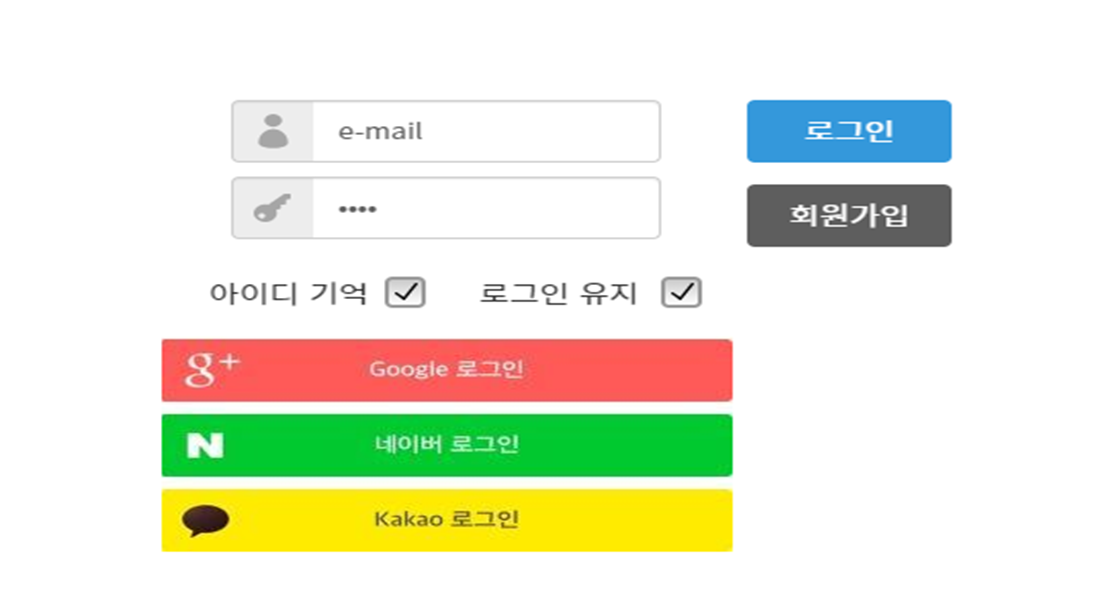
\includegraphics[width=17.00cm]{./Figure/Analysis/Display/login.png}} \\
    \hline
\end{longtable}

\par\
\par\
\textbf{2. 데이터 구성 항목}

\begin{longtable}
    {
        |>{\centering\hspace{0pt}}m{0.150\linewidth}
        |>{\centering\hspace{0pt}}m{0.180\linewidth}
        |>{\centering\hspace{0pt}}m{0.060\linewidth}
        |>{\centering\hspace{0pt}}m{0.110\linewidth}
        |>{\hspace{0pt}}m{0.150\linewidth}
        |>{\arraybackslash\hspace{0pt}}m{0.190\linewidth}|
    } 
    \hline
    \rowcolor{maize} 항목명(한글) & 컨트롤(영문) & 필수 & 수정여부 & \centering{설명} & \centering{비고/제약사항} \endhead 
    \hline
    아이디 & userId & Y & Y & 사용자 아이디 입력 & 특수문자 입력 제한 \\
    \hline
    비밀번호 & password & Y & Y & 사용자 비밀번호 입력 & 영문자와 숫자를 반드시 혼용할 것 \\
    \hline
    아이디 기억 & idSave & N & Y & 사이트 재접속 시 가장 최근에 사용했던 Id 미리 입력 & 로그인을 성공했던 Id만 기억 \\
    \hline
    로그인 유지 & loginSave & N & Y & 직접 로그아웃을 하지 않을 경우 사이트를 꺼도 재접속 시 로그아웃되지 않음 &  \\
    \hline
\end{longtable}

\par\
\par\
\par\
\par\
\par\
\par\
\textbf{3. 처리 로직}

\arrayrulecolor{black}
\begin{longtable}
    {
        |>{\hspace{0pt}}m{0.145\linewidth}
        |>{\hspace{0pt}}m{0.140\linewidth}
        |>{\hspace{0pt}}m{0.300\linewidth}
        |>{\hspace{0pt}}m{0.140\linewidth}
        |>{\hspace{0pt}}m{0.140\linewidth}|} 
    \hline
    \rowcolor{maize} 
    \multicolumn{1}{
        |>{\centering\hspace{0pt}}m{0.145\linewidth}|}{{\cellcolor{maize}}} 
        & \multicolumn{1}{>{\centering\hspace{0pt}}m{0.140\linewidth}|}{입력값/파라미터} 
        & \multicolumn{1}{>{\centering\hspace{0pt}}m{0.300\linewidth}|}{처리내용} 
        & \multicolumn{1}{>{\centering\hspace{0pt}}m{0.140\linewidth}|}{출력/처리결과} 
        & \multicolumn{1}{>{\centering\arraybackslash\hspace{0pt}}m{0.140\linewidth}|}{{\cellcolor{maize}}} \\* 
    \hhline{|>{\arrayrulecolor{maize}}->{\arrayrulecolor{black}}|--->{\arrayrulecolor{maize}}->{\arrayrulecolor{black}}|}
    \rowcolor{maize} 
        \multicolumn{1}{|>{\Centering\hspace{0pt}}m{0.145\linewidth}|}{\multirow{-2}{=}{\cellcolor{maize}\Centering{}이벤트명}} 
        & \multicolumn{1}{>{\Centering\hspace{0pt}}m{0.140\linewidth}|}{시작 JSP} 
        & \multicolumn{1}{>{\Centering\hspace{0pt}}m{0.300\linewidth}|}{프리젠테이션 레이어 설계} 
        & \multicolumn{1}{>{\Centering\hspace{0pt}}m{0.140\linewidth}|}{출력 JSP} 
        & \multicolumn{1}{>{\Centering\hspace{0pt}}m{0.140\linewidth}|}{\multirow{-2}{=}{\cellcolor{maize}\Centering{}비고}} \endhead
    \hline
    \multirow{4}{=}{Client 요청시(onLoad()시)} &  & \multirow{2}{=}{} &  &  \\* 
     \arrayrulecolor[rgb]{0.8,0.8,0.8}\cline{2-2}\arrayrulecolor[rgb]{0.8,0.8,0.8}\cline{4-4}
     &  &  &  &  \\* 
    \arrayrulecolor{black}\cline{2-5}
     & \multicolumn{1}{>{\hspace{0pt}}m{0.140\linewidth}|}{로그인 UI} & \multicolumn{1}{>{\hspace{0pt}}m{0.300\linewidth}|}{Path : URI} & 로그인 UI &  \\* 
     \arrayrulecolor[rgb]{0.8,0.8,0.8}\cline{2-2}\arrayrulecolor{black}\cline{3-3}\arrayrulecolor[rgb]{0.8,0.8,0.8}\cline{4-4}\arrayrulecolor{black}
     &  & \multicolumn{1}{>{\hspace{0pt}}m{0.300\linewidth}|}{Controller : 회원관리Ctrl} &  &  \\* 
    \arrayrulecolor{black}\hline

    \multirow{4}{=}{로그인.onClick()} & 아이디, 비밀번호 & \multirow{2}{=}{입력된 아이디와 비밀번호가 유효한지 검사하여 로그인 여부 확인} & 입력 데이터에 맞는 계정으로 로그인 된 상태로 메인화면UI 이동 & \multirow{4}{=}{필수 입력 사항을 입력하지 않거나 인증번호가 틀렸을 경우 재입력 요구 팝업창 출력} \\* 
     \arrayrulecolor[rgb]{0.8,0.8,0.8}\cline{2-2}\arrayrulecolor[rgb]{0.8,0.8,0.8}\cline{4-4}
     &  &  &  &  \\* 
    \arrayrulecolor{black}\cline{2-4}
     & \multicolumn{1}{>{\hspace{0pt}}m{0.140\linewidth}|}{로그인 UI} & \multicolumn{1}{>{\hspace{0pt}}m{0.300\linewidth}|}{Path : URI} & 메인화면 UI &  \\* 
     \arrayrulecolor[rgb]{0.8,0.8,0.8}\cline{2-2}\arrayrulecolor{black}\cline{3-3}\arrayrulecolor[rgb]{0.8,0.8,0.8}\cline{4-4}\arrayrulecolor{black}
     &  & Controller : 회원관리Ctrl &  &  \\ 
    \arrayrulecolor{black}\hline

    \multirow{5}{=}{Google 로그인.onClick()} & 기록번호 & \multirow{2}{=}{구글 계정 선택 화면으로 Navigation, 계정 선택이 완료 된 후 회원가입 UI로 Navigation} & Google 계정 선택 화면 이동 &  \\* 
     \arrayrulecolor[rgb]{0.8,0.8,0.8}\cline{2-2}\arrayrulecolor[rgb]{0.8,0.8,0.8}\cline{4-4}
     &  &  &  &  \\* 
    \arrayrulecolor{black}\cline{2-5}
     & \multicolumn{1}{>{\hspace{0pt}}m{0.140\linewidth}|}{로그인 UI} & \multicolumn{1}{>{\hspace{0pt}}m{0.300\linewidth}|}{Path : URI} & Google 계정 선택 화면 &  \\* 
     \arrayrulecolor[rgb]{0.8,0.8,0.8}\cline{2-2}\arrayrulecolor{black}\cline{3-3}\arrayrulecolor[rgb]{0.8,0.8,0.8}\cline{4-4}\arrayrulecolor{black}
     &  & Controller : 회원관리Ctrl &  &  \\ 
    \arrayrulecolor{black}\hline

    \multirow{5}{=}{Naver로그인.onClick()} & 기록번호 & \multirow{2}{=}{네이버 계정 연동 동의 화면으로 Navigation, 연동 동의가 완료 된 후 회원가입 UI로 Navigation} & Naver 계정 연동 동의 화면 이동 &  \\* 
     \arrayrulecolor[rgb]{0.8,0.8,0.8}\cline{2-2}\arrayrulecolor[rgb]{0.8,0.8,0.8}\cline{4-4}
     &  &  &  &  \\* 
    \arrayrulecolor{black}\cline{2-5}
     & \multicolumn{1}{>{\hspace{0pt}}m{0.140\linewidth}|}{로그인 UI} & \multicolumn{1}{>{\hspace{0pt}}m{0.300\linewidth}|}{Path : URI} & Naver 계정 연동 동의 화면 &  \\* 
     \arrayrulecolor[rgb]{0.8,0.8,0.8}\cline{2-2}\arrayrulecolor{black}\cline{3-3}\arrayrulecolor[rgb]{0.8,0.8,0.8}\cline{4-4}\arrayrulecolor{black}
     &  & Controller : 회원관리Ctrl &  &  \\ 
    \arrayrulecolor{black}\hline

    \multirow{5}{=}{Kakao로그인.onClick()} & 닉네임 & \multirow{2}{=}{카카오계정 연동 동의 화면으로 Navigation,연동 동의가 완료 된 후 회원가입 UI로 Navigation} & Kakao 계정 연동 동의 화면 이동 &  \\* 
     \arrayrulecolor[rgb]{0.8,0.8,0.8}\cline{2-2}\arrayrulecolor[rgb]{0.8,0.8,0.8}\cline{4-4}
     &  &  &  &  \\* 
    \arrayrulecolor{black}\cline{2-5}
     & \multicolumn{1}{>{\hspace{0pt}}m{0.140\linewidth}|}{로그인 UI} & \multicolumn{1}{>{\hspace{0pt}}m{0.300\linewidth}|}{Path : URI} & Kakao 계정 연동 동의 화면 &  \\* 
     \arrayrulecolor[rgb]{0.8,0.8,0.8}\cline{2-2}\arrayrulecolor{black}\cline{3-3}\arrayrulecolor[rgb]{0.8,0.8,0.8}\cline{4-4}\arrayrulecolor{black}
     &  & Controller : 회원관리Ctrl &  &  \\ 
    \arrayrulecolor{black}\hline

    \multirow{4}{=}{회원가입.onClick()} & 닉네임 & \multirow{2}{=}{회원가입화면으로 Navigation} & 회원가입화면 이동 &  \\* 
     \arrayrulecolor[rgb]{0.8,0.8,0.8}\cline{2-2}\arrayrulecolor[rgb]{0.8,0.8,0.8}\cline{4-4}
     &  &  &  &  \\* 
    \arrayrulecolor{black}\cline{2-5}
     & \multicolumn{1}{>{\hspace{0pt}}m{0.140\linewidth}|}{로그인 UI} & \multicolumn{1}{>{\hspace{0pt}}m{0.300\linewidth}|}{Path : URI} & 회원가입UI &  \\* 
     \arrayrulecolor[rgb]{0.8,0.8,0.8}\cline{2-2}\arrayrulecolor{black}\cline{3-3}\arrayrulecolor[rgb]{0.8,0.8,0.8}\cline{4-4}\arrayrulecolor{black}
     &  & Controller : 회원관리Ctrl &  &  \\ 
    \arrayrulecolor{black}\hline
\end{longtable}
\newpage

\footnotesize
\begin{longtable}[htp]
        {
            |>{\centering\hspace{0pt}}m{0.140\linewidth}
            |>{\hspace{0pt}}m{0.300\linewidth}
            |>{\centering\hspace{0pt}}m{0.140\linewidth}
            |>{\hspace{0pt}}m{0.300\linewidth}|
        } 
    \hline
    \multicolumn{4}{|c|}{{\cellcolor{maize}}{\Large\textbf{화 면 정 의 서}}} \\ 
    \hline
    시스템명 & TeulDa & 작성일 & 2021.01.02 \\ 
    \hline
    업 무 명 & 회원관리 & 작성자 & 김채경 \\ 
    \hline
    화면 ID & myProfile & 화면명 & 개인프로필 조회 \\ 
    \hline
    화면개요 & \multicolumn{3}{l|}{개인 프로필 화면} \\ 
    \hline
    \multicolumn{4}{|c|}{}\\
    \multicolumn{4}{|l|}{\textbf{1. 화면 레이아웃}} \\ 
    \multicolumn{4}{|l|}{\hspace{6pt}{자신의 개인 프로필}} \\ 
    \multicolumn{4}{|c|}{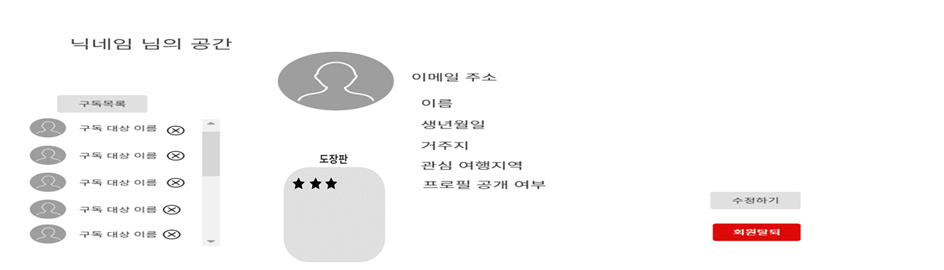
\includegraphics[width=17.00cm]{./Figure/Analysis/Display/myprofile.png}} \\

    \multicolumn{4}{|l|}{\hspace{6pt}{타인의 개인 프로필}} \\ 
    \multicolumn{4}{|c|}{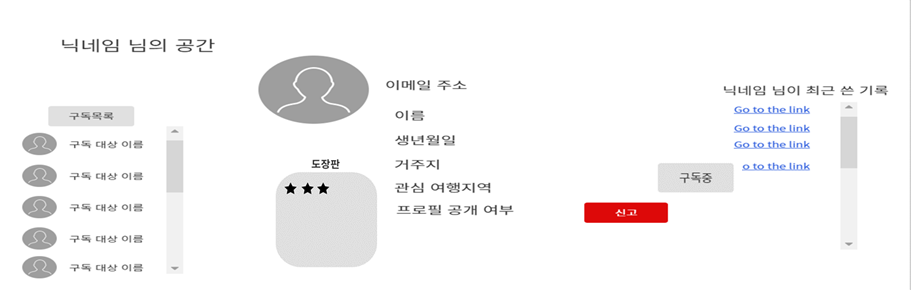
\includegraphics[width=17.00cm]{./Figure/Analysis/Display/profile.png}} \\

    \hline
\end{longtable}

\textbf{2. 데이터 구성 항목}

\begin{longtable}
    {
        |>{\centering\hspace{0pt}}m{0.150\linewidth}
        |>{\centering\hspace{0pt}}m{0.180\linewidth}
        |>{\centering\hspace{0pt}}m{0.060\linewidth}
        |>{\centering\hspace{0pt}}m{0.110\linewidth}
        |>{\hspace{0pt}}m{0.150\linewidth}
        |>{\arraybackslash\hspace{0pt}}m{0.190\linewidth}|
    } 
    \hline
    \rowcolor{maize} 항목명(한글) & 컨트롤(영문) & 필수 & 수정여부 & \centering{설명} & \centering{비고/제약사항} \endhead 
    \hline
    아이디 & userId & Y & N & 사용자 아이디(이메일) 출력 & 소셜 로그인 시 입력 불가 \\ 
    \hline
    이름 & userName & Y & Y & 사용자 이름 출력 & 특수문자 사용 불가 \\ 
    \hline
    닉네임 & userNick & Y & N & 사용자 닉네임 출력 & 특수문자 사용 불가 \\ 
    \hline
    생년월일 & birthday & Y & Y & 사용자 생년월일 출력 &  \\ 
    \hline
    거주지 & resi & Y & Y & 사용자 거주지 출력 &  \\ 
    \hline
    관심 여행지역 & interest & Y & Y & 사용자 관심지역 출력 &  \\ 
    \hline
    프로필 사진 & myPhoto & Y & Y & 사용자 프로필사진 출력 &  \\ 
    \hline
    프로필 공개 여부 & openPro & N & Y & 해당 계정을 다른 사용자에 공개 할 지 여부 &  \\ 
    \hline
    구독자 목록 & subscribeList & N & Y & 사용자가 구독하는 목록 출력 &  \\ 
    \hline
    도장 id & stampId & N & N & 랜드마크 방문 인증시 얻은 도장을 식별하기 위한 id &  \\ 
    \hline
    도장 이름 & stamp & N & N & 랜드마크 방문 인증 시 도장이 하나씩 추가 &  \\ 
    \hline
    계정 상태 & status & Y & N & 활성화, 정지, 휴면 세가지 상태로 구분 & Hidden,계정 생성시 `활성화' default \\ 
    \hline
    계정 상태 변경일 & statusDate & Y & N & 계정 상태가 정지, 혹은 휴면상태로 바뀌었을 때 각 상태에 따른 조치 자동화를 위한 데이터 & Hidden,정지 상태에서 2주 경과시 자동 활성화휴면상태에서 1달 이내로 접속 시 자동 활성화, 그렇지 않을 경우 데이터 삭제 \\ 
    \hline
    역할 & role & Y & N & 사용자의 계정 역할 구분 & Hidden, 사용자와 관리자 구분 \\
    \hline
\end{longtable}

\textbf{3. 처리 로직}

\arrayrulecolor{black}
\begin{longtable}
    {
        |>{\hspace{0pt}}m{0.145\linewidth}
        |>{\hspace{0pt}}m{0.140\linewidth}
        |>{\hspace{0pt}}m{0.300\linewidth}
        |>{\hspace{0pt}}m{0.140\linewidth}
        |>{\hspace{0pt}}m{0.140\linewidth}|} 
    \hline
    \rowcolor{maize} 
    \multicolumn{1}{
        |>{\centering\hspace{0pt}}m{0.145\linewidth}|}{{\cellcolor{maize}}} 
        & \multicolumn{1}{>{\centering\hspace{0pt}}m{0.140\linewidth}|}{입력값/파라미터} 
        & \multicolumn{1}{>{\centering\hspace{0pt}}m{0.300\linewidth}|}{처리내용} 
        & \multicolumn{1}{>{\centering\hspace{0pt}}m{0.140\linewidth}|}{출력/처리결과} 
        & \multicolumn{1}{>{\centering\arraybackslash\hspace{0pt}}m{0.140\linewidth}|}{{\cellcolor{maize}}} \\* 
    \hhline{|>{\arrayrulecolor{maize}}->{\arrayrulecolor{black}}|--->{\arrayrulecolor{maize}}->{\arrayrulecolor{black}}|}
    \rowcolor{maize} 
        \multicolumn{1}{|>{\Centering\hspace{0pt}}m{0.145\linewidth}|}{\multirow{-2}{=}{\cellcolor{maize}\Centering{}이벤트명}} 
        & \multicolumn{1}{>{\Centering\hspace{0pt}}m{0.140\linewidth}|}{시작 JSP} 
        & \multicolumn{1}{>{\Centering\hspace{0pt}}m{0.300\linewidth}|}{프리젠테이션 레이어 설계} 
        & \multicolumn{1}{>{\Centering\hspace{0pt}}m{0.140\linewidth}|}{출력 JSP} 
        & \multicolumn{1}{>{\Centering\hspace{0pt}}m{0.140\linewidth}|}{\multirow{-2}{=}{\cellcolor{maize}\Centering{}비고}} \endhead
    \hline
    \multirow{4}{=}{Client 요청시(onLoad()시)} &  & \multirow{2}{=}{} &  &  \\* 
     \arrayrulecolor[rgb]{0.8,0.8,0.8}\cline{2-2}\arrayrulecolor[rgb]{0.8,0.8,0.8}\cline{4-4}
     &  &  &  &  \\* 
    \arrayrulecolor{black}\cline{2-5}
     & \multicolumn{1}{>{\hspace{0pt}}m{0.140\linewidth}|}{개인프로필 조회 UI} & \multicolumn{1}{>{\hspace{0pt}}m{0.300\linewidth}|}{Path : URI} & 로그인 UI &  \\* 
     \arrayrulecolor[rgb]{0.8,0.8,0.8}\cline{2-2}\arrayrulecolor{black}\cline{3-3}\arrayrulecolor[rgb]{0.8,0.8,0.8}\cline{4-4}\arrayrulecolor{black}
     &  & \multicolumn{1}{>{\hspace{0pt}}m{0.300\linewidth}|}{Controller : 회원관리Ctrl} &  &  \\* 
    \arrayrulecolor{black}\hline

    \multirow{4}{=}{수정하기.onClick()} & 이메일 & \multirow{2}{=}{정보 입력사항을 수정할 수 있는 개인프로필 수정 UI로 Navigation} &  &  \\* 
     \arrayrulecolor[rgb]{0.8,0.8,0.8}\cline{2-2}\arrayrulecolor[rgb]{0.8,0.8,0.8}\cline{4-4}
     &  &  &  &  \\* 
    \arrayrulecolor{black}\cline{2-5}
     & \multicolumn{1}{>{\hspace{0pt}}m{0.140\linewidth}|}{개인프로필 조회 UI} & \multicolumn{1}{>{\hspace{0pt}}m{0.300\linewidth}|}{Path : URI} & 개인프로필 수정 UI &  \\* 
     \arrayrulecolor[rgb]{0.8,0.8,0.8}\cline{2-2}\arrayrulecolor{black}\cline{3-3}\arrayrulecolor[rgb]{0.8,0.8,0.8}\cline{4-4}\arrayrulecolor{black}
     &  & Controller : 회원관리Ctrl &  &  \\ 
    \arrayrulecolor{black}\hline

    \multirow{4}{=}{회원탈퇴.onClick()} & 이메일 & \multirow{2}{=}{이메일 인증 UI로 Navigation} &  & \multirow{4}{=}{이메일 인증 UI로 이동하기 전, 탈퇴의사를 다시 한번 묻는 팝업창 출력/본인계정에서만 사용 가능} \\* 
     \arrayrulecolor[rgb]{0.8,0.8,0.8}\cline{2-2}\arrayrulecolor[rgb]{0.8,0.8,0.8}\cline{4-4}
     &  &  &  &  \\* 
    \arrayrulecolor{black}\cline{2-4}
     & \multicolumn{1}{>{\hspace{0pt}}m{0.140\linewidth}|}{개인프로필 조회 UI(본인)} & \multicolumn{1}{>{\hspace{0pt}}m{0.300\linewidth}|}{Path : URI} & 이메일 인증 UI	 &  \\* 
     \arrayrulecolor[rgb]{0.8,0.8,0.8}\cline{2-2}\arrayrulecolor{black}\cline{3-3}\arrayrulecolor[rgb]{0.8,0.8,0.8}\cline{4-4}\arrayrulecolor{black}
     &  & Controller : 회원관리Ctrl &  &  \\ 
    \arrayrulecolor{black}\hline

    \multirow{4}{=}{구독버튼.onClick()} & 내 닉네임, 구독대상 닉네임 & \multirow{2}{=}{해당 버튼을 눌러서 구독/구독 취소} &  & \multirow{4}{=}{버튼명 구독하지 않은 상태: 구독하기 구독한 상태: 구독중} \\* 
     \arrayrulecolor[rgb]{0.8,0.8,0.8}\cline{2-2}\arrayrulecolor[rgb]{0.8,0.8,0.8}\cline{4-4}
     &  &  &  &  \\* 
    \arrayrulecolor{black}\cline{2-4}
     & \multicolumn{1}{>{\hspace{0pt}}m{0.140\linewidth}|}{개인프로필 조회 UI(타인)} & \multicolumn{1}{>{\hspace{0pt}}m{0.300\linewidth}|}{Path : URI} & 개인프로필 UI(타인) &  \\* 
     \arrayrulecolor[rgb]{0.8,0.8,0.8}\cline{2-2}\arrayrulecolor{black}\cline{3-3}\arrayrulecolor[rgb]{0.8,0.8,0.8}\cline{4-4}\arrayrulecolor{black}
     &  & Controller : 커뮤니티관리Ctrl &  &  \\ 
    \arrayrulecolor{black}\hline

    \multirow{4}{=}{신고하기.onClick()} & 신고자 이메일, 신고대상 이메일 & \multirow{2}{=}{계정 신고화면 UI로 Navigation} &  & \multirow{5}{=}{타인계정에서만 사용 가능} \\* 
     \arrayrulecolor[rgb]{0.8,0.8,0.8}\cline{2-2}\arrayrulecolor[rgb]{0.8,0.8,0.8}\cline{4-4}
     &  &  &  &  \\* 
    \arrayrulecolor{black}\cline{2-4}
     & \multicolumn{1}{>{\hspace{0pt}}m{0.140\linewidth}|}{개인프로필 조회 UI(타인)} & \multicolumn{1}{>{\hspace{0pt}}m{0.300\linewidth}|}{Path : URI} & 계정 신고화면 UI &  \\* 
     \arrayrulecolor[rgb]{0.8,0.8,0.8}\cline{2-2}\arrayrulecolor{black}\cline{3-3}\arrayrulecolor[rgb]{0.8,0.8,0.8}\cline{4-4}\arrayrulecolor{black}
     &  & Controller : 회원관리Ctrl &  &  \\ 
    \arrayrulecolor{black}\hline

    \multirow{4}{=}{구독자.onClick()} & 구독대상 닉네임 & \multirow{2}{=}{해당 계정의 개인프로필 UI로 Navigation} &  &  \\* 
     \arrayrulecolor[rgb]{0.8,0.8,0.8}\cline{2-2}\arrayrulecolor[rgb]{0.8,0.8,0.8}\cline{4-4}
     &  &  &  &  \\* 
    \arrayrulecolor{black}\cline{2-5}
     & \multicolumn{1}{>{\hspace{0pt}}m{0.140\linewidth}|}{개인프로필 조회 UI} & \multicolumn{1}{>{\hspace{0pt}}m{0.300\linewidth}|}{Path : URI} & 개인프로필 UI(타인) &  \\* 
     \arrayrulecolor[rgb]{0.8,0.8,0.8}\cline{2-2}\arrayrulecolor{black}\cline{3-3}\arrayrulecolor[rgb]{0.8,0.8,0.8}\cline{4-4}\arrayrulecolor{black}
     &  & Controller : 회원관리Ctrl &  &  \\ 
    \arrayrulecolor{black}\hline

    \multirow{4}{=}{구독취소.onClick()} & 내 닉네임, 구독대상 닉네임 & \multirow{2}{=}{더 이상 구독 하고 싶지 않은 사용자목록 옆의 x아이콘을 눌러 구독 취소, 취소시 페이지를 reload하여 갱신해서 출력} &  & \multirow{5}{=}{개인계정에서만 사용 가능} \\* 
     \arrayrulecolor[rgb]{0.8,0.8,0.8}\cline{2-2}\arrayrulecolor[rgb]{0.8,0.8,0.8}\cline{4-4}
     &  &  &  &  \\* 
    \arrayrulecolor{black}\cline{2-4}
     & \multicolumn{1}{>{\hspace{0pt}}m{0.140\linewidth}|}{개인프로필 조회 UI(본인)} & \multicolumn{1}{>{\hspace{0pt}}m{0.300\linewidth}|}{Path : URI} & 개인프로필 UI(개인) &  \\* 
     \arrayrulecolor[rgb]{0.8,0.8,0.8}\cline{2-2}\arrayrulecolor{black}\cline{3-3}\arrayrulecolor[rgb]{0.8,0.8,0.8}\cline{4-4}\arrayrulecolor{black}
     &  & Controller : 회원관리Ctrl &  &  \\ 
    \arrayrulecolor{black}\hline

    \multirow{4}{=}{최근 쓴 기록.onClick()} & 대상 닉네임 & \multirow{2}{=}{해당 기록 상세조회UI로 Navigation} &  & \multirow{4}{=}{타인계정에서만 사용 가능} \\* 
     \arrayrulecolor[rgb]{0.8,0.8,0.8}\cline{2-2}\arrayrulecolor[rgb]{0.8,0.8,0.8}\cline{4-4}
     &  &  &  &  \\* 
    \arrayrulecolor{black}\cline{2-4}
     & \multicolumn{1}{>{\hspace{0pt}}m{0.140\linewidth}|}{개인프로필 조회 UI(타인)} & \multicolumn{1}{>{\hspace{0pt}}m{0.300\linewidth}|}{Path : URI} & 기록상세조회 UI(타인) &  \\* 
     \arrayrulecolor[rgb]{0.8,0.8,0.8}\cline{2-2}\arrayrulecolor{black}\cline{3-3}\arrayrulecolor[rgb]{0.8,0.8,0.8}\cline{4-4}\arrayrulecolor{black}
     &  & Controller : 기록관리Ctrl &  &  \\ 
    \arrayrulecolor{black}\hline

    \multirow{4}{=}{회원목록조회.onClick()} &  & \multirow{2}{=}{회원목록 조회 UI로 Navigation} &  & \multirow{4}{=}{관리자계정에서만 사용 가능} \\* 
     \arrayrulecolor[rgb]{0.8,0.8,0.8}\cline{2-2}\arrayrulecolor[rgb]{0.8,0.8,0.8}\cline{4-4}
     &  &  &  &  \\* 
    \arrayrulecolor{black}\cline{2-4}
     & \multicolumn{1}{>{\hspace{0pt}}m{0.140\linewidth}|}{개인프로필 조회 UI(관리자)} & \multicolumn{1}{>{\hspace{0pt}}m{0.300\linewidth}|}{Path : URI} & 회원목록 조회UI &  \\* 
     \arrayrulecolor[rgb]{0.8,0.8,0.8}\cline{2-2}\arrayrulecolor{black}\cline{3-3}\arrayrulecolor[rgb]{0.8,0.8,0.8}\cline{4-4}\arrayrulecolor{black}
     &  & Controller : 회원관리Ctrl &  &  \\ 
    \arrayrulecolor{black}\hline

    \multirow{4}{=}{블랙리스트 목록 조회.onClick()} &  & \multirow{2}{=}{신고 횟수가 10회 이상인 사용자 목록만 출력하는 블랙리스트 목록 UI로 Navigation} &  & \multirow{4}{=}{관리자계정에서만 사용 가능} \\* 
     \arrayrulecolor[rgb]{0.8,0.8,0.8}\cline{2-2}\arrayrulecolor[rgb]{0.8,0.8,0.8}\cline{4-4}
     &  &  &  &  \\* 
    \arrayrulecolor{black}\cline{2-4}
     & \multicolumn{1}{>{\hspace{0pt}}m{0.140\linewidth}|}{개인프로필 조회 UI(관리자))} & \multicolumn{1}{>{\hspace{0pt}}m{0.300\linewidth}|}{Path : URI} & 블랙리스트목록 조회 UI &  \\* 
     \arrayrulecolor[rgb]{0.8,0.8,0.8}\cline{2-2}\arrayrulecolor{black}\cline{3-3}\arrayrulecolor[rgb]{0.8,0.8,0.8}\cline{4-4}\arrayrulecolor{black}
     &  & Controller : 회원관리Ctrl &  &  \\ 
    \arrayrulecolor{black}\hline
\end{longtable}
\newpage

\footnotesize
\begin{longtable}[htp]
        {
            |>{\centering\hspace{0pt}}m{0.140\linewidth}
            |>{\hspace{0pt}}m{0.300\linewidth}
            |>{\centering\hspace{0pt}}m{0.140\linewidth}
            |>{\hspace{0pt}}m{0.300\linewidth}|
        } 
    \hline
    \multicolumn{4}{|c|}{{\cellcolor{maize}}{\Large\textbf{화 면 정 의 서}}} \\ 
    \hline
    시스템명 & TeulDa & 작성일 & 2021.01.02 \\ 
    \hline
    업 무 명 & 회원관리 & 작성자 & 김채경 \\ 
    \hline
    화면 ID & emailCon & 화면명 & 이메일 인증 \\ 
    \hline
    화면개요 & \multicolumn{3}{l|}{이메일 인증안내 화면} \\ 
    \hline
    \multicolumn{4}{|c|}{}\\
    \multicolumn{4}{|l|}{\textbf{1. 화면 레이아웃}} \\ 
    % \multicolumn{4}{|l|}{\hspace{6pt}{자사회원 가입시}} \\ 
    % \multicolumn{4}{|c|}{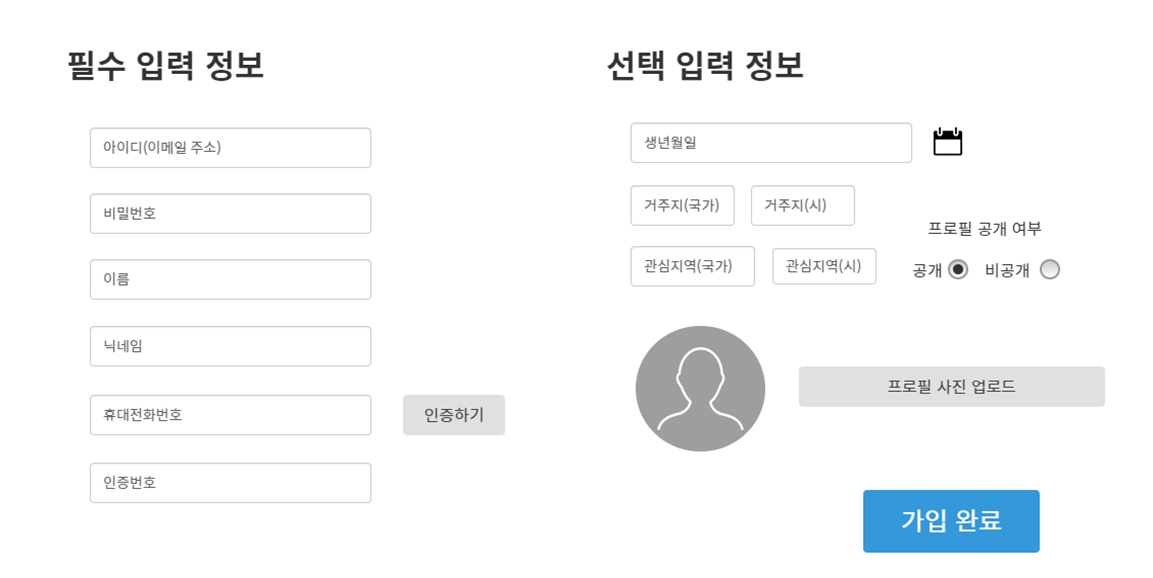
\includegraphics[width=17.00cm]{./Figure/Analysis/Display/addusert.png}} \\

    % \multicolumn{4}{|l|}{\hspace{6pt}{소셜회원 가입시}} \\ 
    \multicolumn{4}{|c|}{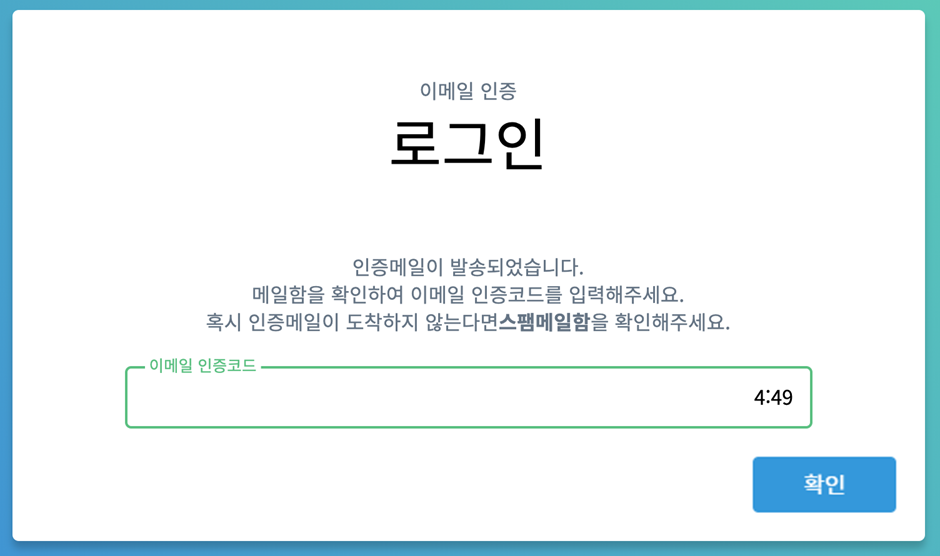
\includegraphics[width=17.00cm]{./Figure/Analysis/Display/email.png}} \\

    \hline
\end{longtable}

\textbf{2. 데이터 구성 항목}

\begin{longtable}
    {
        |>{\centering\hspace{0pt}}m{0.150\linewidth}
        |>{\centering\hspace{0pt}}m{0.180\linewidth}
        |>{\centering\hspace{0pt}}m{0.060\linewidth}
        |>{\centering\hspace{0pt}}m{0.110\linewidth}
        |>{\hspace{0pt}}m{0.150\linewidth}
        |>{\arraybackslash\hspace{0pt}}m{0.190\linewidth}|
    } 
    \hline
    \rowcolor{maize} 항목명(한글) & 컨트롤(영문) & 필수 & 수정여부 & \centering{설명} & \centering{비고/제약사항} \endhead 
    \hline
    인증코드 & conCode & Y & N & 인증메일에 적힌 코드 입력 & 세션시간 5분 제공 \\ 
    \hline
\end{longtable}

\textbf{3. 처리 로직}

\arrayrulecolor{black}
\begin{longtable}
    {
        |>{\hspace{0pt}}m{0.145\linewidth}
        |>{\hspace{0pt}}m{0.140\linewidth}
        |>{\hspace{0pt}}m{0.300\linewidth}
        |>{\hspace{0pt}}m{0.140\linewidth}
        |>{\hspace{0pt}}m{0.140\linewidth}|} 
    \hline
    \rowcolor{maize} 
    \multicolumn{1}{
        |>{\centering\hspace{0pt}}m{0.145\linewidth}|}{{\cellcolor{maize}}} 
        & \multicolumn{1}{>{\centering\hspace{0pt}}m{0.140\linewidth}|}{입력값/파라미터} 
        & \multicolumn{1}{>{\centering\hspace{0pt}}m{0.300\linewidth}|}{처리내용} 
        & \multicolumn{1}{>{\centering\hspace{0pt}}m{0.140\linewidth}|}{출력/처리결과} 
        & \multicolumn{1}{>{\centering\arraybackslash\hspace{0pt}}m{0.140\linewidth}|}{{\cellcolor{maize}}} \\* 
    \hhline{|>{\arrayrulecolor{maize}}->{\arrayrulecolor{black}}|--->{\arrayrulecolor{maize}}->{\arrayrulecolor{black}}|}
    \rowcolor{maize} 
        \multicolumn{1}{|>{\Centering\hspace{0pt}}m{0.145\linewidth}|}{\multirow{-2}{=}{\cellcolor{maize}\Centering{}이벤트명}} 
        & \multicolumn{1}{>{\Centering\hspace{0pt}}m{0.140\linewidth}|}{시작 JSP} 
        & \multicolumn{1}{>{\Centering\hspace{0pt}}m{0.300\linewidth}|}{프리젠테이션 레이어 설계} 
        & \multicolumn{1}{>{\Centering\hspace{0pt}}m{0.140\linewidth}|}{출력 JSP} 
        & \multicolumn{1}{>{\Centering\hspace{0pt}}m{0.140\linewidth}|}{\multirow{-2}{=}{\cellcolor{maize}\Centering{}비고}} \endhead
    \hline
    \multirow{4}{=}{Client 요청시(onLoad()시)} &  & \multirow{2}{=}{} &  &  \\* 
     \arrayrulecolor[rgb]{0.8,0.8,0.8}\cline{2-2}\arrayrulecolor[rgb]{0.8,0.8,0.8}\cline{4-4}
     &  &  &  &  \\* 
    \arrayrulecolor{black}\cline{2-5}
     & \multicolumn{1}{>{\hspace{0pt}}m{0.140\linewidth}|}{이메일 인증 UI} & \multicolumn{1}{>{\hspace{0pt}}m{0.300\linewidth}|}{Path : URI} & 이메일 인증 UI &  \\* 
     \arrayrulecolor[rgb]{0.8,0.8,0.8}\cline{2-2}\arrayrulecolor{black}\cline{3-3}\arrayrulecolor[rgb]{0.8,0.8,0.8}\cline{4-4}\arrayrulecolor{black}
     &  & \multicolumn{1}{>{\hspace{0pt}}m{0.300\linewidth}|}{Controller : 회원관리Ctrl} &  &  \\* 
    \arrayrulecolor{black}\hline

    \multirow{4}{=}{확인.onClick()} & 인증코드 & \multirow{2}{=}{인증코드가 유효한지 검사} & 회원가입 완료 화면 이동 & \multirow{4}{=}{인증 실패시 재입력 요구 에러 메시지 표현} \\* 
     \arrayrulecolor[rgb]{0.8,0.8,0.8}\cline{2-2}\arrayrulecolor[rgb]{0.8,0.8,0.8}\cline{4-4}
     &  &  &  &  \\* 
    \arrayrulecolor{black}\cline{2-4}
     & \multicolumn{1}{>{\hspace{0pt}}m{0.140\linewidth}|}{이메일 인증 UI} & \multicolumn{1}{>{\hspace{0pt}}m{0.300\linewidth}|}{Path : URI} & 회원가입 완료 UI &  \\* 
     \arrayrulecolor[rgb]{0.8,0.8,0.8}\cline{2-2}\arrayrulecolor{black}\cline{3-3}\arrayrulecolor[rgb]{0.8,0.8,0.8}\cline{4-4}\arrayrulecolor{black}
     &  & Controller : 회원관리Ctrl &  &  \\ 
    \arrayrulecolor{black}\hline
\end{longtable}
\newpage


\footnotesize
\begin{longtable}[htp]
        {
            |>{\centering\hspace{0pt}}m{0.140\linewidth}
            |>{\hspace{0pt}}m{0.300\linewidth}
            |>{\centering\hspace{0pt}}m{0.140\linewidth}
            |>{\hspace{0pt}}m{0.300\linewidth}|
        } 
    \hline
    \multicolumn{4}{|c|}{{\cellcolor{maize}}{\Large\textbf{화 면 정 의 서}}} \\ 
    \hline
    시스템명 & TeulDa & 작성일 & 2021.01.02 \\ 
    \hline
    업 무 명 & 회원관리 & 작성자 & 김채경 \\ 
    \hline
    화면 ID & successUser & 화면명 & 회원가입 완료 \\ 
    \hline
    화면개요 & \multicolumn{3}{l|}{회원가입 완료} \\ 
    \hline
    \multicolumn{4}{|c|}{}\\
    \multicolumn{4}{|l|}{\textbf{1. 화면 레이아웃}} \\ 
    % \multicolumn{4}{|l|}{\hspace{6pt}{자사회원 가입시}} \\ 
    % \multicolumn{4}{|c|}{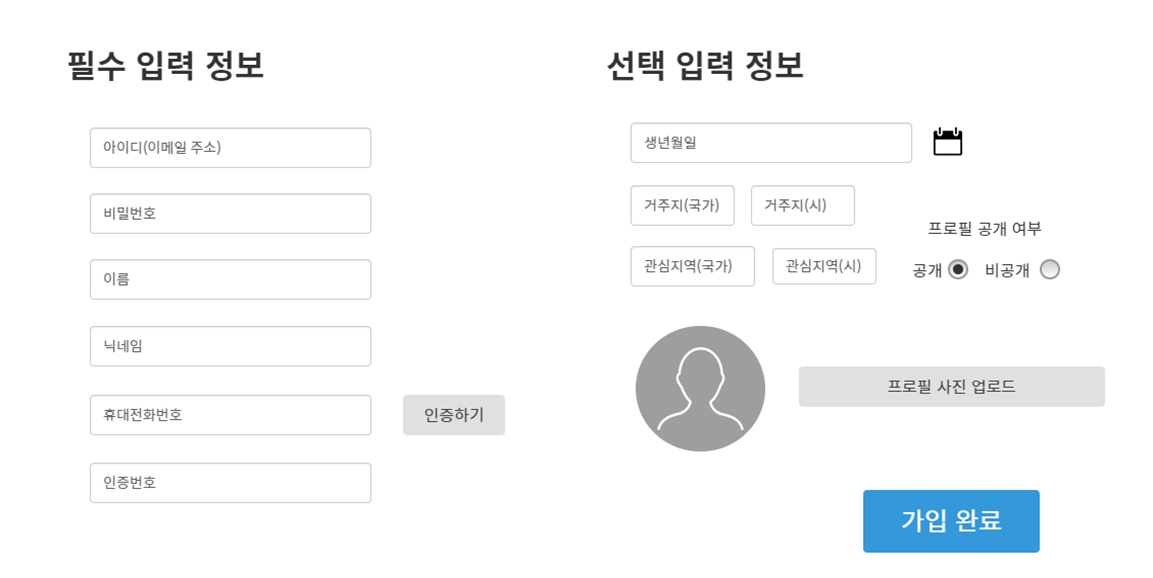
\includegraphics[width=17.00cm]{./Figure/Analysis/Display/addusert.png}} \\

    % \multicolumn{4}{|l|}{\hspace{6pt}{소셜회원 가입시}} \\ 
    \multicolumn{4}{|c|}{
\includegraphics[width=17.00cm]{./Figure/Analysis/Display/complete.png}} \\

    \hline
\end{longtable}

\textbf{2. 데이터 구성 항목}

\begin{longtable}
    {
        |>{\centering\hspace{0pt}}m{0.150\linewidth}
        |>{\centering\hspace{0pt}}m{0.180\linewidth}
        |>{\centering\hspace{0pt}}m{0.060\linewidth}
        |>{\centering\hspace{0pt}}m{0.110\linewidth}
        |>{\hspace{0pt}}m{0.150\linewidth}
        |>{\arraybackslash\hspace{0pt}}m{0.190\linewidth}|
    } 
    \hline
    \rowcolor{maize} 항목명(한글) & 컨트롤(영문) & 필수 & 수정여부 & \centering{설명} & \centering{비고/제약사항} \endhead 
    \hline
     &  &  &  &  &  \\ 
    \hline
\end{longtable}

\textbf{3. 처리 로직}

\arrayrulecolor{black}
\begin{longtable}
    {
        |>{\hspace{0pt}}m{0.145\linewidth}
        |>{\hspace{0pt}}m{0.140\linewidth}
        |>{\hspace{0pt}}m{0.300\linewidth}
        |>{\hspace{0pt}}m{0.140\linewidth}
        |>{\hspace{0pt}}m{0.140\linewidth}|} 
    \hline
    \rowcolor{maize} 
    \multicolumn{1}{
        |>{\centering\hspace{0pt}}m{0.145\linewidth}|}{{\cellcolor{maize}}} 
        & \multicolumn{1}{>{\centering\hspace{0pt}}m{0.140\linewidth}|}{입력값/파라미터} 
        & \multicolumn{1}{>{\centering\hspace{0pt}}m{0.300\linewidth}|}{처리내용} 
        & \multicolumn{1}{>{\centering\hspace{0pt}}m{0.140\linewidth}|}{출력/처리결과} 
        & \multicolumn{1}{>{\centering\arraybackslash\hspace{0pt}}m{0.140\linewidth}|}{{\cellcolor{maize}}} \\* 
    \hhline{|>{\arrayrulecolor{maize}}->{\arrayrulecolor{black}}|--->{\arrayrulecolor{maize}}->{\arrayrulecolor{black}}|}
    \rowcolor{maize} 
        \multicolumn{1}{|>{\Centering\hspace{0pt}}m{0.145\linewidth}|}{\multirow{-2}{=}{\cellcolor{maize}\Centering{}이벤트명}} 
        & \multicolumn{1}{>{\Centering\hspace{0pt}}m{0.140\linewidth}|}{시작 JSP} 
        & \multicolumn{1}{>{\Centering\hspace{0pt}}m{0.300\linewidth}|}{프리젠테이션 레이어 설계} 
        & \multicolumn{1}{>{\Centering\hspace{0pt}}m{0.140\linewidth}|}{출력 JSP} 
        & \multicolumn{1}{>{\Centering\hspace{0pt}}m{0.140\linewidth}|}{\multirow{-2}{=}{\cellcolor{maize}\Centering{}비고}} \endhead
    \hline
    \multirow{4}{=}{Client 요청시(onLoad()시)} &  & \multirow{2}{=}{} &  &  \\* 
     \arrayrulecolor[rgb]{0.8,0.8,0.8}\cline{2-2}\arrayrulecolor[rgb]{0.8,0.8,0.8}\cline{4-4}
     &  &  &  &  \\* 
    \arrayrulecolor{black}\cline{2-5}
     & \multicolumn{1}{>{\hspace{0pt}}m{0.140\linewidth}|}{회원가입 완료 UI} & \multicolumn{1}{>{\hspace{0pt}}m{0.300\linewidth}|}{Path : URI} & 회원가입 완료 UI &  \\* 
     \arrayrulecolor[rgb]{0.8,0.8,0.8}\cline{2-2}\arrayrulecolor{black}\cline{3-3}\arrayrulecolor[rgb]{0.8,0.8,0.8}\cline{4-4}\arrayrulecolor{black}
     &  & \multicolumn{1}{>{\hspace{0pt}}m{0.300\linewidth}|}{Controller : 회원관리Ctrl} &  &  \\* 
    \arrayrulecolor{black}\hline

    \multirow{4}{=}{좋아요.onClick()} &  & \multirow{2}{=}{정보 입력사항을 수정할 수 있는 개인프로필 수정 UI로 Navigation} & 로그인 한 채로 메인페이지로 이동 &  \\* 
     \arrayrulecolor[rgb]{0.8,0.8,0.8}\cline{2-2}\arrayrulecolor[rgb]{0.8,0.8,0.8}\cline{4-4}
     &  &  &  &  \\* 
    \arrayrulecolor{black}\cline{2-5}
     & \multicolumn{1}{>{\hspace{0pt}}m{0.140\linewidth}|}{회원가입 완료 UI} & \multicolumn{1}{>{\hspace{0pt}}m{0.300\linewidth}|}{Path : URI} & 메인 UI &  \\* 
     \arrayrulecolor[rgb]{0.8,0.8,0.8}\cline{2-2}\arrayrulecolor{black}\cline{3-3}\arrayrulecolor[rgb]{0.8,0.8,0.8}\cline{4-4}\arrayrulecolor{black}
     &  & Controller : 회원관리Ctrl &  &  \\ 
    \arrayrulecolor{black}\hline
\end{longtable}
\newpage

\footnotesize
\begin{longtable}[htp]
        {
            |>{\centering\hspace{0pt}}m{0.140\linewidth}
            |>{\hspace{0pt}}m{0.300\linewidth}
            |>{\centering\hspace{0pt}}m{0.140\linewidth}
            |>{\hspace{0pt}}m{0.300\linewidth}|
        } 
    \hline
    \multicolumn{4}{|c|}{{\cellcolor{maize}}{\Large\textbf{화 면 정 의 서}}} \\ 
    \hline
    시스템명 & TeulDa & 작성일 & 2021.01.02 \\ 
    \hline
    업 무 명 & 회원관리 & 작성자 & 김채경 \\ 
    \hline
    화면 ID & withdrawUser & 화면명 & 회원 탈퇴 \\ 
    \hline
    화면개요 & \multicolumn{3}{l|}{회원 탈퇴 완료 UI} \\ 
    \hline
    \multicolumn{4}{|c|}{}\\
    \multicolumn{4}{|l|}{\textbf{1. 화면 레이아웃}} \\ 
    % \multicolumn{4}{|l|}{\hspace{6pt}{자사회원 가입시}} \\ 
    % \multicolumn{4}{|c|}{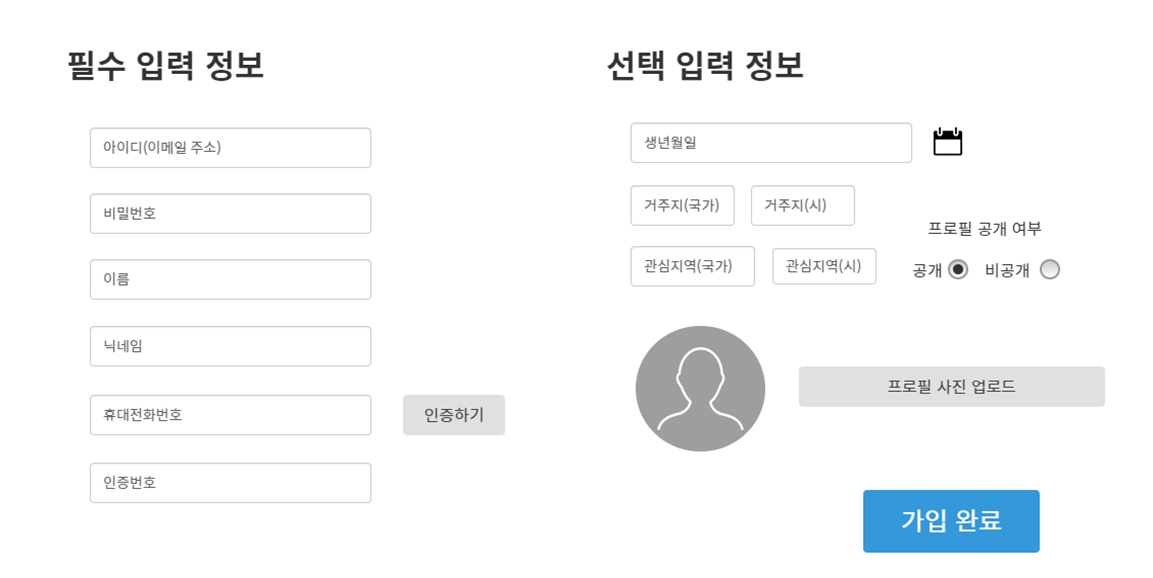
\includegraphics[width=17.00cm]{./Figure/Analysis/Display/addusert.png}} \\

    % \multicolumn{4}{|l|}{\hspace{6pt}{소셜회원 가입시}} \\ 
    \multicolumn{4}{|c|}{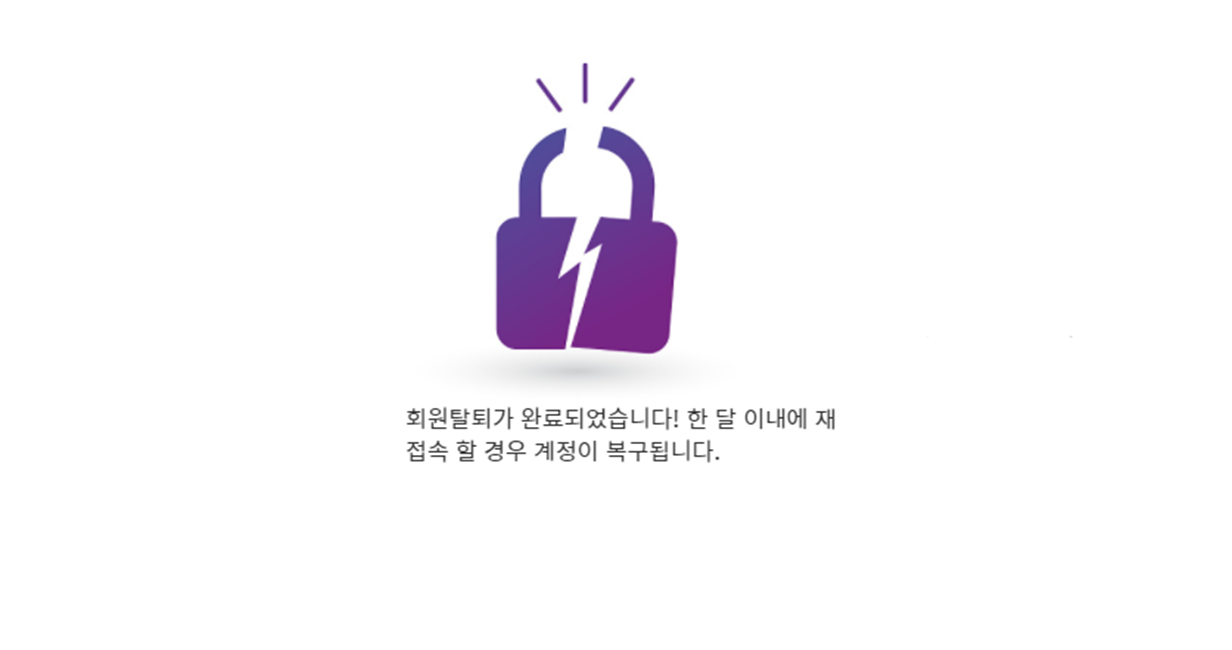
\includegraphics[width=17.00cm]{./Figure/Analysis/Display/withdrawUser.png}} \\

    \hline
\end{longtable}

\textbf{2. 데이터 구성 항목}

\begin{longtable}
    {
        |>{\centering\hspace{0pt}}m{0.150\linewidth}
        |>{\centering\hspace{0pt}}m{0.180\linewidth}
        |>{\centering\hspace{0pt}}m{0.060\linewidth}
        |>{\centering\hspace{0pt}}m{0.110\linewidth}
        |>{\hspace{0pt}}m{0.150\linewidth}
        |>{\arraybackslash\hspace{0pt}}m{0.190\linewidth}|
    } 
    \hline
    \rowcolor{maize} 항목명(한글) & 컨트롤(영문) & 필수 & 수정여부 & \centering{설명} & \centering{비고/제약사항} \endhead 
    \hline
     &  &  &  &  &  \\
    \hline
\end{longtable}

\textbf{3. 처리 로직}

\arrayrulecolor{black}
\begin{longtable}
    {
        |>{\hspace{0pt}}m{0.145\linewidth}
        |>{\hspace{0pt}}m{0.140\linewidth}
        |>{\hspace{0pt}}m{0.300\linewidth}
        |>{\hspace{0pt}}m{0.140\linewidth}
        |>{\hspace{0pt}}m{0.140\linewidth}|} 
    \hline
    \rowcolor{maize} 
    \multicolumn{1}{
        |>{\centering\hspace{0pt}}m{0.145\linewidth}|}{{\cellcolor{maize}}} 
        & \multicolumn{1}{>{\centering\hspace{0pt}}m{0.140\linewidth}|}{입력값/파라미터} 
        & \multicolumn{1}{>{\centering\hspace{0pt}}m{0.300\linewidth}|}{처리내용} 
        & \multicolumn{1}{>{\centering\hspace{0pt}}m{0.140\linewidth}|}{출력/처리결과} 
        & \multicolumn{1}{>{\centering\arraybackslash\hspace{0pt}}m{0.140\linewidth}|}{{\cellcolor{maize}}} \\* 
    \hhline{|>{\arrayrulecolor{maize}}->{\arrayrulecolor{black}}|--->{\arrayrulecolor{maize}}->{\arrayrulecolor{black}}|}
    \rowcolor{maize} 
        \multicolumn{1}{|>{\Centering\hspace{0pt}}m{0.145\linewidth}|}{\multirow{-2}{=}{\cellcolor{maize}\Centering{}이벤트명}} 
        & \multicolumn{1}{>{\Centering\hspace{0pt}}m{0.140\linewidth}|}{시작 JSP} 
        & \multicolumn{1}{>{\Centering\hspace{0pt}}m{0.300\linewidth}|}{프리젠테이션 레이어 설계} 
        & \multicolumn{1}{>{\Centering\hspace{0pt}}m{0.140\linewidth}|}{출력 JSP} 
        & \multicolumn{1}{>{\Centering\hspace{0pt}}m{0.140\linewidth}|}{\multirow{-2}{=}{\cellcolor{maize}\Centering{}비고}} \endhead
    \hline
    \multirow{4}{=}{Client 요청시(onLoad()시)} &  & \multirow{2}{=}{} &  & \multirow{4}{=}{탈퇴한 계정은 자동 로그아웃 되며 휴면상태로 변경. 한달내로 재접속이 없을시 완전히 삭제, 한 달내로 재접속시 활성화상태로 복구} \\* 
     \arrayrulecolor[rgb]{0.8,0.8,0.8}\cline{2-2}\arrayrulecolor[rgb]{0.8,0.8,0.8}\cline{4-4}
     &  &  &  &  \\* 
    \arrayrulecolor{black}\cline{2-4}
     & \multicolumn{1}{>{\hspace{0pt}}m{0.140\linewidth}|}{회원탈퇴 완료 UI} & \multicolumn{1}{>{\hspace{0pt}}m{0.300\linewidth}|}{Path : URI} & 회원탈퇴 완료 UI &  \\* 
     \arrayrulecolor[rgb]{0.8,0.8,0.8}\cline{2-2}\arrayrulecolor{black}\cline{3-3}\arrayrulecolor[rgb]{0.8,0.8,0.8}\cline{4-4}\arrayrulecolor{black}
     &  & \multicolumn{1}{>{\hspace{0pt}}m{0.300\linewidth}|}{Controller : 회원관리Ctrl} &  &  \\* 
    \arrayrulecolor{black}\hline
\end{longtable}
\newpage

\footnotesize
\begin{longtable}[htp]
        {
            |>{\centering\hspace{0pt}}m{0.140\linewidth}
            |>{\hspace{0pt}}m{0.300\linewidth}
            |>{\centering\hspace{0pt}}m{0.140\linewidth}
            |>{\hspace{0pt}}m{0.300\linewidth}|
        } 
    \hline
    \multicolumn{4}{|c|}{{\cellcolor{maize}}{\Large\textbf{화 면 정 의 서}}} \\ 
    \hline
    시스템명 & TeulDa & 작성일 & 2021.01.02 \\ 
    \hline
    업 무 명 & 회원관리 & 작성자 & 김채경 \\ 
    \hline
    화면 ID & myProfileUpdate & 화면명 & 개인프로필 수정 \\ 
    \hline
    화면개요 & \multicolumn{3}{l|}{개인 프로필 수정 화면} \\ 
    \hline
    \multicolumn{4}{|c|}{}\\
    \multicolumn{4}{|l|}{\textbf{1. 화면 레이아웃}} \\ 
    % \multicolumn{4}{|l|}{\hspace{6pt}{자사회원 가입시}} \\ 
    % \multicolumn{4}{|c|}{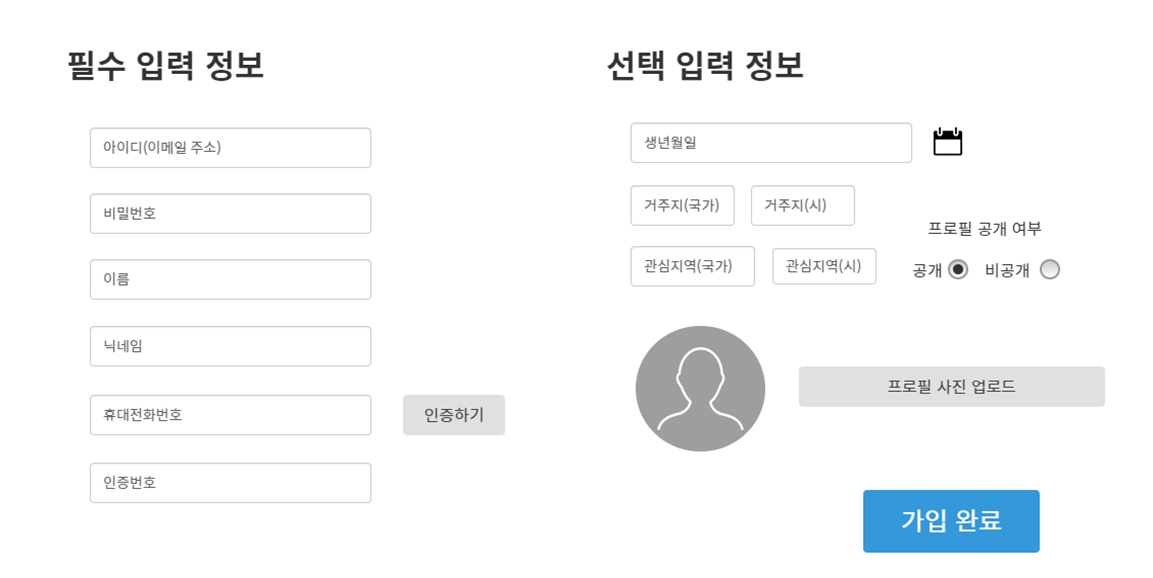
\includegraphics[width=17.00cm]{./Figure/Analysis/Display/addusert.png}} \\

    % \multicolumn{4}{|l|}{\hspace{6pt}{소셜회원 가입시}} \\ 
    \multicolumn{4}{|c|}{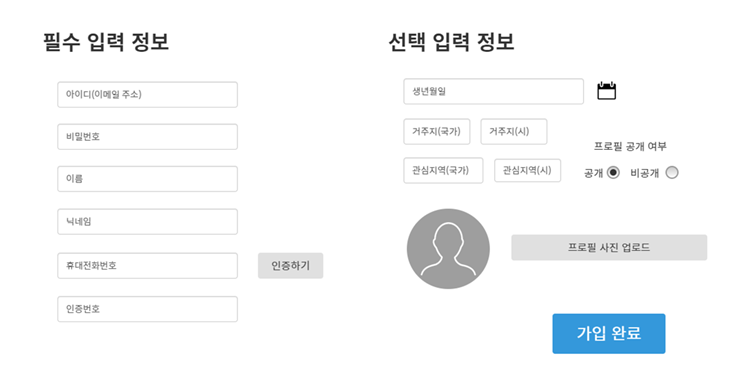
\includegraphics[width=17.00cm]{./Figure/Analysis/Display/myProfileUpdate.png}} \\

    \hline
\end{longtable}

\textbf{2. 데이터 구성 항목}

\begin{longtable}
    {
        |>{\centering\hspace{0pt}}m{0.150\linewidth}
        |>{\centering\hspace{0pt}}m{0.180\linewidth}
        |>{\centering\hspace{0pt}}m{0.060\linewidth}
        |>{\centering\hspace{0pt}}m{0.110\linewidth}
        |>{\hspace{0pt}}m{0.150\linewidth}
        |>{\arraybackslash\hspace{0pt}}m{0.190\linewidth}|
    } 
    \hline
    \rowcolor{maize} 항목명(한글) & 컨트롤(영문) & 필수 & 수정여부 & \centering{설명} & \centering{비고/제약사항} \endhead 
    \hline
    비밀번호 & password & Y & Y & 사용자 비밀번호 입력 & 6자 이상 입력, 소셜로그인 시 입력불가 \\
    \hline
    휴대전화번호 & userPhone & Y & Y & 사용자 휴대전화번호 입력 & 숫자만 입력 가능 \\ 
    \hline
    생년월일 & birthday & Y & Y & 사용자 생년월일 입력 &  \\ 
    \hline
    거주지 & resi & Y & Y & 사용자 거주지 입력 &  \\ 
    \hline
    관심 여행지역 & interest & Y & Y & 사용자 관심지역 입력 &  \\ 
    \hline
    프로필 사진 & myPhoto & Y & Y & 사용자 프로필사진 업로드 &  \\ 
    \hline
    인증번호 & conNumber & Y & Y & 전화번호 변경 시 본인 핸드폰번호 인증~ & ~세션시간 5분 제공 \\ 
    \hline
    프로필 공개 여부 & openPro & N & Y & 해당 계정을 다른 사용자에 공개 할 지 여부 결정 &  \\ 
    \hline
    계정 상태 & status & Y & N & 활성화, 정지, 휴면 세가지 상태로 구분 & Hidden,계정 생성시 '활성화' default \\ 
    \hline
    계정 상태 변경일 & statusDate & Y & N & 계정 상태가 정지, 혹은 휴면상태로 바뀌었을 때 각 상태에 따른 조치 자동화를 위한 데이터 & Hidden,정지 상태에서 2주 경과시 자동 활성화 휴면상태에서 1달 이내로 접속 시 자동 활성화, 그렇지 않을 경우 데이터 삭제 \\ 
    \hline
    역할 & role & Y & Y & 사용자의 계정 역할 구분 & Hidden, 사용자와 관리자 구분 \\
    \hline
\end{longtable}

\textbf{3. 처리 로직}

\arrayrulecolor{black}
\begin{longtable}
    {
        |>{\hspace{0pt}}m{0.145\linewidth}
        |>{\hspace{0pt}}m{0.140\linewidth}
        |>{\hspace{0pt}}m{0.300\linewidth}
        |>{\hspace{0pt}}m{0.140\linewidth}
        |>{\hspace{0pt}}m{0.140\linewidth}|} 
    \hline
    \rowcolor{maize} 
    \multicolumn{1}{
        |>{\centering\hspace{0pt}}m{0.145\linewidth}|}{{\cellcolor{maize}}} 
        & \multicolumn{1}{>{\centering\hspace{0pt}}m{0.140\linewidth}|}{입력값/파라미터} 
        & \multicolumn{1}{>{\centering\hspace{0pt}}m{0.300\linewidth}|}{처리내용} 
        & \multicolumn{1}{>{\centering\hspace{0pt}}m{0.140\linewidth}|}{출력/처리결과} 
        & \multicolumn{1}{>{\centering\arraybackslash\hspace{0pt}}m{0.140\linewidth}|}{{\cellcolor{maize}}} \\* 
    \hhline{|>{\arrayrulecolor{maize}}->{\arrayrulecolor{black}}|--->{\arrayrulecolor{maize}}->{\arrayrulecolor{black}}|}
    \rowcolor{maize} 
        \multicolumn{1}{|>{\Centering\hspace{0pt}}m{0.145\linewidth}|}{\multirow{-2}{=}{\cellcolor{maize}\Centering{}이벤트명}} 
        & \multicolumn{1}{>{\Centering\hspace{0pt}}m{0.140\linewidth}|}{시작 JSP} 
        & \multicolumn{1}{>{\Centering\hspace{0pt}}m{0.300\linewidth}|}{프리젠테이션 레이어 설계} 
        & \multicolumn{1}{>{\Centering\hspace{0pt}}m{0.140\linewidth}|}{출력 JSP} 
        & \multicolumn{1}{>{\Centering\hspace{0pt}}m{0.140\linewidth}|}{\multirow{-2}{=}{\cellcolor{maize}\Centering{}비고}} \endhead
    \hline
    \multirow{4}{=}{Client 요청시(onLoad()시)} &  & \multirow{2}{=}{} &  &  \\* 
     \arrayrulecolor[rgb]{0.8,0.8,0.8}\cline{2-2}\arrayrulecolor[rgb]{0.8,0.8,0.8}\cline{4-4}
     &  &  &  &  \\* 
    \arrayrulecolor{black}\cline{2-5}
     & \multicolumn{1}{>{\hspace{0pt}}m{0.140\linewidth}|}{updateUser.jsp} & \multicolumn{1}{>{\hspace{0pt}}m{0.300\linewidth}|}{Path : /user/updateUser : POST} & updateUser.jsp &  \\* 
     \arrayrulecolor[rgb]{0.8,0.8,0.8}\cline{2-2}\arrayrulecolor{black}\cline{3-3}\arrayrulecolor[rgb]{0.8,0.8,0.8}\cline{4-4}\arrayrulecolor{black}
     &  & \multicolumn{1}{>{\hspace{0pt}}m{0.300\linewidth}|}{Controller : com.teulda.web.user.UserCont
     roller.updateUser()} &  &  \\* 
    \arrayrulecolor{black}\hline

    \multirow{4}{=}{인증하기.onClick()} & 전화번호 & \multirow{2}{=}{미리 입력한 전화번호로 인증번호문자 전송 및 팝업창으로 인증문자전송 안내} &  & \multirow{4.5}{=}{변경하는 전화번호가 본인 전화번호인지 확인하는 절차} \\* 
     \arrayrulecolor[rgb]{0.8,0.8,0.8}\cline{2-2}\arrayrulecolor[rgb]{0.8,0.8,0.8}\cline{4-4}
     &  &  &  &  \\* 
    \arrayrulecolor{black}\cline{2-4}
     & \multicolumn{1}{>{\hspace{0pt}}m{0.140\linewidth}|}{updateUser.jsp} & \multicolumn{1}{>{\hspace{0pt}}m{0.300\linewidth}|}{Path : /user/updateUser : POST} & updateUser.jsp &  \\* 
     \arrayrulecolor[rgb]{0.8,0.8,0.8}\cline{2-2}\arrayrulecolor{black}\cline{3-3}\arrayrulecolor[rgb]{0.8,0.8,0.8}\cline{4-4}\arrayrulecolor{black}
     &  & Controller : com.teulda.web.user.UserCont
     roller.checkPhone() &  &  \\ 
    \arrayrulecolor{black}\hline

    \multirow{4}{=}{프로필 사진 업로드.onClick()} & 사진 파일 & \multirow{2}{=}{프로필 사진 업로드 팝업창 출력} &  &  \\* 
     \arrayrulecolor[rgb]{0.8,0.8,0.8}\cline{2-2}\arrayrulecolor[rgb]{0.8,0.8,0.8}\cline{4-4}
     &  &  &  &  \\* 
    \arrayrulecolor{black}\cline{2-5}
     & \multicolumn{1}{>{\hspace{0pt}}m{0.140\linewidth}|}{updateUser.jsp} & \multicolumn{1}{>{\hspace{0pt}}m{0.300\linewidth}|}{Path : /user/updateUser : POST} & updateUser.jsp &  \\* 
     \arrayrulecolor[rgb]{0.8,0.8,0.8}\cline{2-2}\arrayrulecolor{black}\cline{3-3}\arrayrulecolor[rgb]{0.8,0.8,0.8}\cline{4-4}\arrayrulecolor{black}
     &  & Controller : com.teulda.web.user.UserCont
     roller.updateUser() &  &  \\ 
    \arrayrulecolor{black}\hline

    \multirow{4}{=}{수정완료.onClick()} &  & \multirow{2}{=}{데이터를 업데이트하고 개인프로필조회 UI로 Navigation} & 개인프로필 조회화면으로 이동 & \multirow{4.5}{=}{필수 입력 사항을 입력하지 않거나 인증번호가 틀렸을 경우 재입력 요구 팝업창 출력} \\* 
     \arrayrulecolor[rgb]{0.8,0.8,0.8}\cline{2-2}\arrayrulecolor[rgb]{0.8,0.8,0.8}\cline{4-4}
     &  &  &  &  \\* 
    \arrayrulecolor{black}\cline{2-4}
     & \multicolumn{1}{>{\hspace{0pt}}m{0.140\linewidth}|}{updateUser.jsp} & \multicolumn{1}{>{\hspace{0pt}}m{0.300\linewidth}|}{Path : /user/updateUser : POST} & getUser.jsp &  \\* 
     \arrayrulecolor[rgb]{0.8,0.8,0.8}\cline{2-2}\arrayrulecolor{black}\cline{3-3}\arrayrulecolor[rgb]{0.8,0.8,0.8}\cline{4-4}\arrayrulecolor{black}
     &  & Controller : com.teulda.web.user.UserCont
     roller.updateUser() &  &  \\ 
    \arrayrulecolor{black}\hline
\end{longtable}
\newpage

\footnotesize
\begin{longtable}[htp]
        {
            |>{\centering\hspace{0pt}}m{0.140\linewidth}
            |>{\hspace{0pt}}m{0.300\linewidth}
            |>{\centering\hspace{0pt}}m{0.140\linewidth}
            |>{\hspace{0pt}}m{0.300\linewidth}|
        } 
    \hline
    \multicolumn{4}{|c|}{{\cellcolor{maize}}{\Large\textbf{화 면 정 의 서}}} \\ 
    \hline
    시스템명 & TeulDa & 작성일 & 2021.01.02 \\ 
    \hline
    업 무 명 & 회원관리 & 작성자 & 김채경 \\ 
    \hline
    화면 ID & report & 화면명 & 계정 신고화면 \\ 
    \hline
    화면개요 & \multicolumn{3}{l|}{계정 신고화면} \\ 
    \hline
    \multicolumn{4}{|c|}{}\\
    \multicolumn{4}{|l|}{\textbf{1. 화면 레이아웃}} \\ 
    % \multicolumn{4}{|l|}{\hspace{6pt}{자사회원 가입시}} \\ 
    % \multicolumn{4}{|c|}{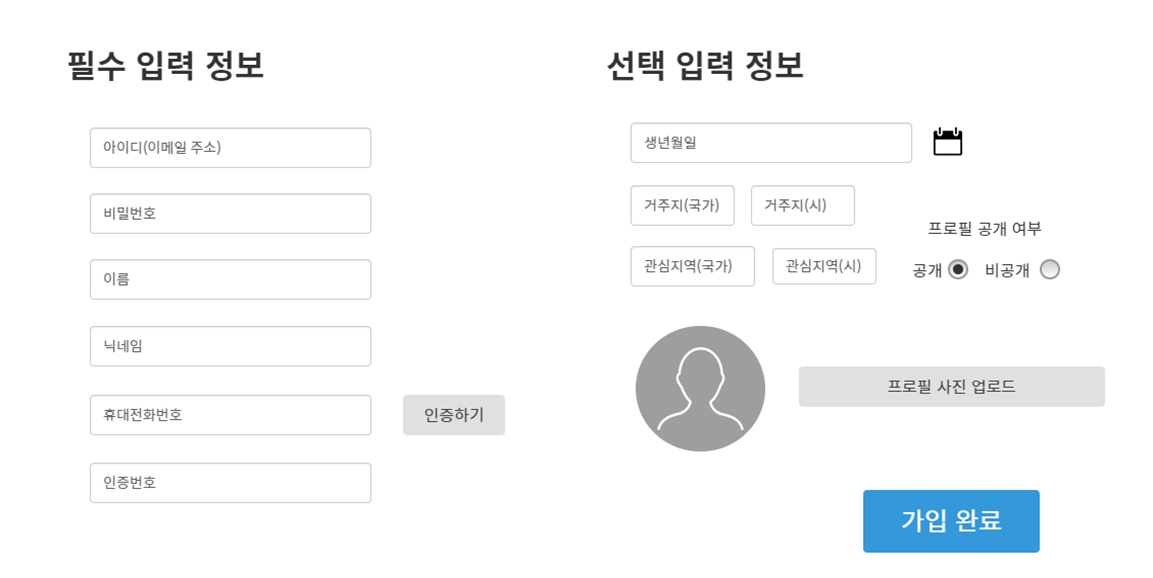
\includegraphics[width=17.00cm]{./Figure/Analysis/Display/addusert.png}} \\

    % \multicolumn{4}{|l|}{\hspace{6pt}{소셜회원 가입시}} \\ 
    \multicolumn{4}{|c|}{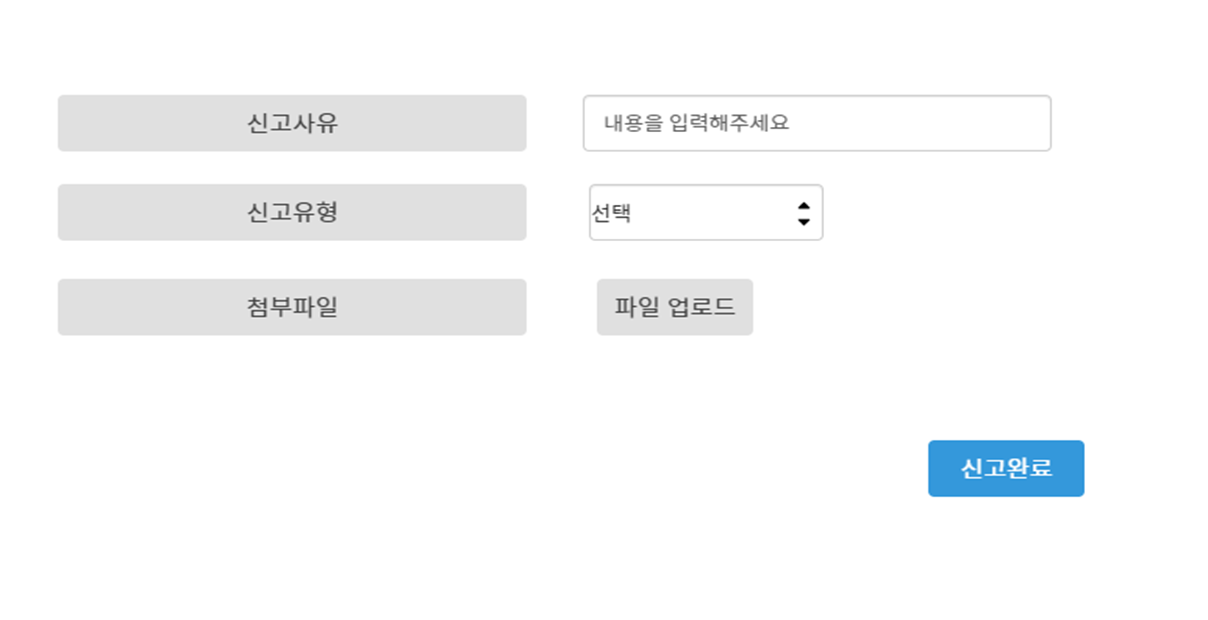
\includegraphics[width=17.00cm]{./Figure/Analysis/Display/report.png}} \\

    \hline
\end{longtable}

\textbf{2. 데이터 구성 항목}

\begin{longtable}
    {
        |>{\centering\hspace{0pt}}m{0.150\linewidth}
        |>{\centering\hspace{0pt}}m{0.180\linewidth}
        |>{\centering\hspace{0pt}}m{0.060\linewidth}
        |>{\centering\hspace{0pt}}m{0.110\linewidth}
        |>{\hspace{0pt}}m{0.150\linewidth}
        |>{\arraybackslash\hspace{0pt}}m{0.190\linewidth}|
    } 
    \hline
    \rowcolor{maize} 항목명(한글) & 컨트롤(영문) & 필수 & 수정여부 & \centering{설명} & \centering{비고/제약사항} \endhead 
    \hline
    항목명(한글) & 컨트롤(영문) & 필수 & 수정여부 & 설명 & 비고/제약사항 \\
    \hline
    신고사유 & reason & Y & Y & 신고사유 입력 & 글자제한 50자 \\ 
    \hline
    증빙자료 & proof & Y & Y & 사용자 생년월일 입력 &  \\ 
    \hline
    신고날짜 & reportDate & Y & N & 신고한 날짜 등록 & Hidden \\
    \hline
\end{longtable}

\textbf{3. 처리 로직}

\arrayrulecolor{black}
\begin{longtable}
    {
        |>{\hspace{0pt}}m{0.145\linewidth}
        |>{\hspace{0pt}}m{0.140\linewidth}
        |>{\hspace{0pt}}m{0.300\linewidth}
        |>{\hspace{0pt}}m{0.140\linewidth}
        |>{\hspace{0pt}}m{0.140\linewidth}|} 
    \hline
    \rowcolor{maize} 
    \multicolumn{1}{
        |>{\centering\hspace{0pt}}m{0.145\linewidth}|}{{\cellcolor{maize}}} 
        & \multicolumn{1}{>{\centering\hspace{0pt}}m{0.140\linewidth}|}{입력값/파라미터} 
        & \multicolumn{1}{>{\centering\hspace{0pt}}m{0.300\linewidth}|}{처리내용} 
        & \multicolumn{1}{>{\centering\hspace{0pt}}m{0.140\linewidth}|}{출력/처리결과} 
        & \multicolumn{1}{>{\centering\arraybackslash\hspace{0pt}}m{0.140\linewidth}|}{{\cellcolor{maize}}} \\* 
    \hhline{|>{\arrayrulecolor{maize}}->{\arrayrulecolor{black}}|--->{\arrayrulecolor{maize}}->{\arrayrulecolor{black}}|}
    \rowcolor{maize} 
        \multicolumn{1}{|>{\Centering\hspace{0pt}}m{0.145\linewidth}|}{\multirow{-2}{=}{\cellcolor{maize}\Centering{}이벤트명}} 
        & \multicolumn{1}{>{\Centering\hspace{0pt}}m{0.140\linewidth}|}{시작 JSP} 
        & \multicolumn{1}{>{\Centering\hspace{0pt}}m{0.300\linewidth}|}{프리젠테이션 레이어 설계} 
        & \multicolumn{1}{>{\Centering\hspace{0pt}}m{0.140\linewidth}|}{출력 JSP} 
        & \multicolumn{1}{>{\Centering\hspace{0pt}}m{0.140\linewidth}|}{\multirow{-2}{=}{\cellcolor{maize}\Centering{}비고}} \endhead
    \hline
    \multirow{4}{=}{Client 요청시(onLoad()시)} &  & \multirow{2}{=}{} &  &  \\* 
     \arrayrulecolor[rgb]{0.8,0.8,0.8}\cline{2-2}\arrayrulecolor[rgb]{0.8,0.8,0.8}\cline{4-4}
     &  &  &  &  \\* 
    \arrayrulecolor{black}\cline{2-5}
     & \multicolumn{1}{>{\hspace{0pt}}m{0.140\linewidth}|}{reportUser.jsp} & \multicolumn{1}{>{\hspace{0pt}}m{0.300\linewidth}|}{Path : /user/reportUser : GET} & reportUser.jsp &  \\* 
     \arrayrulecolor[rgb]{0.8,0.8,0.8}\cline{2-2}\arrayrulecolor{black}\cline{3-3}\arrayrulecolor[rgb]{0.8,0.8,0.8}\cline{4-4}\arrayrulecolor{black}
     &  & \multicolumn{1}{>{\hspace{0pt}}m{0.300\linewidth}|}{Controller : com.teulda.web.user.UserCont
     roller.reportUser()} &  &  \\* 
    \arrayrulecolor{black}\hline

    \multirow{4}{=}{파일업로드.onClick()} & 사진파일 & \multirow{2}{=}{신고사유 증빙자료 첨부} &  &  \\* 
     \arrayrulecolor[rgb]{0.8,0.8,0.8}\cline{2-2}\arrayrulecolor[rgb]{0.8,0.8,0.8}\cline{4-4}
     &  &  &  &  \\* 
    \arrayrulecolor{black}\cline{2-5}
     & \multicolumn{1}{>{\hspace{0pt}}m{0.140\linewidth}|}{reportUser.jsp} & \multicolumn{1}{>{\hspace{0pt}}m{0.300\linewidth}|}{Path : /user/reportUser : GET} & reportUser.jsp &  \\* 
     \arrayrulecolor[rgb]{0.8,0.8,0.8}\cline{2-2}\arrayrulecolor{black}\cline{3-3}\arrayrulecolor[rgb]{0.8,0.8,0.8}\cline{4-4}\arrayrulecolor{black}
     &  & Controller : com.teulda.web.user.UserCont
     roller.reportUser() &  &  \\ 
    \arrayrulecolor{black}\hline

    \multirow{4}{=}{신고완료.onClick()} & 신고사유, 신고유형, 증빙자료, 신고날짜 & \multirow{2}{=}{신고가 완료되었다는 안내창 출력 및 신고한 계정의 개인프로필 UI로 Navigation} & 신고했던 개인프로필 조회화면으로 이동 & \multirow{4}{=}{신고사유 및 신고유형을 입력하지 않았을 경우 입력해달라는 안내창 출력} \\* 
     \arrayrulecolor[rgb]{0.8,0.8,0.8}\cline{2-2}\arrayrulecolor[rgb]{0.8,0.8,0.8}\cline{4-4}
     &  &  &  &  \\* 
    \arrayrulecolor{black}\cline{2-4}
     & \multicolumn{1}{>{\hspace{0pt}}m{0.140\linewidth}|}{reportUser.jsp} & \multicolumn{1}{>{\hspace{0pt}}m{0.300\linewidth}|}{Path : /user/reportUser : POST} & reportUser.jsp &  \\* 
     \arrayrulecolor[rgb]{0.8,0.8,0.8}\cline{2-2}\arrayrulecolor{black}\cline{3-3}\arrayrulecolor[rgb]{0.8,0.8,0.8}\cline{4-4}\arrayrulecolor{black}
     &  & Controller : com.teulda.web.user.UserCont
     roller.reportUser() &  &  \\ 
    \arrayrulecolor{black}\hline
\end{longtable}
\newpage

\footnotesize
\begin{longtable}[htp]
        {
            |>{\centering\hspace{0pt}}m{0.140\linewidth}
            |>{\hspace{0pt}}m{0.300\linewidth}
            |>{\centering\hspace{0pt}}m{0.140\linewidth}
            |>{\hspace{0pt}}m{0.300\linewidth}|
        } 
    \hline
    \multicolumn{4}{|c|}{{\cellcolor{maize}}{\Large\textbf{화 면 정 의 서}}} \\ 
    \hline
    시스템명 & TeulDa & 작성일 & 2021.01.02 \\ 
    \hline
    업 무 명 & 회원관리 & 작성자 & 김채경 \\ 
    \hline
    화면 ID & blacklistList & 화면명 & 블랙리스트 목록 \\ 
    \hline
    화면개요 & \multicolumn{3}{l|}{블랙리스트 목록조회 화면} \\ 
    \hline
    \multicolumn{4}{|c|}{}\\
    \multicolumn{4}{|l|}{\textbf{1. 화면 레이아웃}} \\ 
    % \multicolumn{4}{|l|}{\hspace{6pt}{자사회원 가입시}} \\ 
    % \multicolumn{4}{|c|}{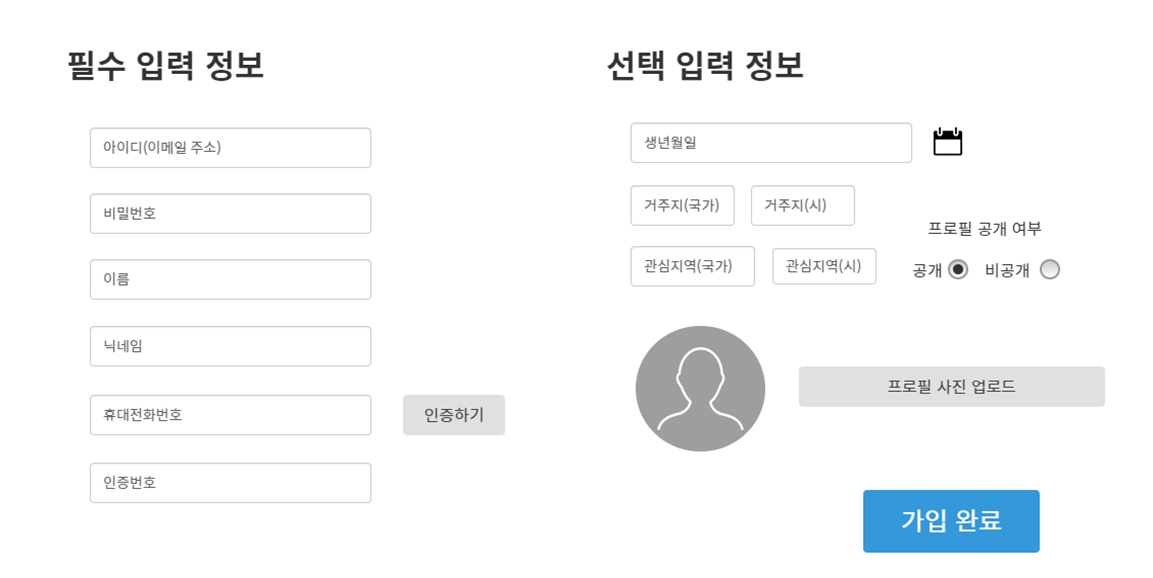
\includegraphics[width=17.00cm]{./Figure/Analysis/Display/addusert.png}} \\

    % \multicolumn{4}{|l|}{\hspace{6pt}{소셜회원 가입시}} \\ 
    \multicolumn{4}{|c|}{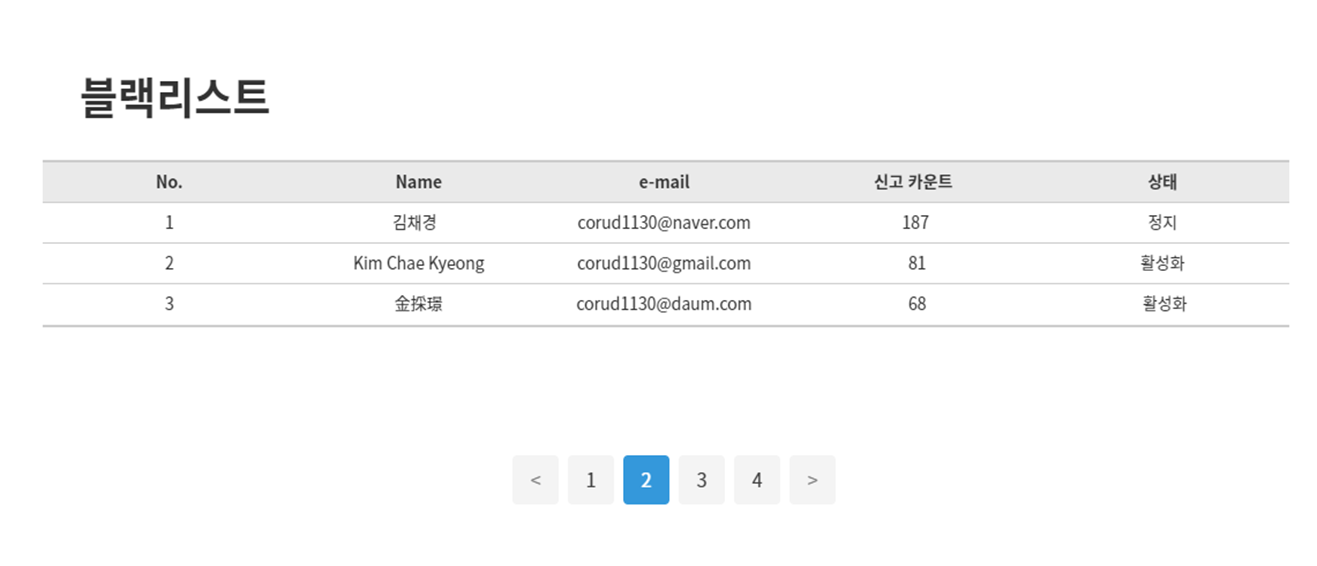
\includegraphics[width=17.00cm]{./Figure/Analysis/Display/blacklistList.png}} \\

    \hline
\end{longtable}

\textbf{2. 데이터 구성 항목}

\begin{longtable}
    {
        |>{\centering\hspace{0pt}}m{0.150\linewidth}
        |>{\centering\hspace{0pt}}m{0.180\linewidth}
        |>{\centering\hspace{0pt}}m{0.060\linewidth}
        |>{\centering\hspace{0pt}}m{0.110\linewidth}
        |>{\hspace{0pt}}m{0.150\linewidth}
        |>{\arraybackslash\hspace{0pt}}m{0.190\linewidth}|
    } 
    \hline
    \rowcolor{maize} 항목명(한글) & 컨트롤(영문) & 필수 & 수정여부 & \centering{설명} & \centering{비고/제약사항} \endhead 
    \hline
    블랙리스트 No & blackListNo & Y & Y & 블랙리스트 유저 넘버링 &  \\ 
    \hline
    이름 & name & Y & Y & 블랙리스트 유저 이름 출력 &  \\ 
    \hline
    이메일 & e-mail & Y & Y & 블랙리스트 유저 이메일 출력 &  \\ 
    \hline
    신고 횟수 & reportCount & Y & Y & 신고당한 횟수 출력 &  \\ 
    \hline
    계정 상태 변경일 & statusDate & Y & N & 계정 상태가 정지, 혹은 휴면상태로 바뀌었을 때 각 상태에 따른 조치 자동화를 위한 데이터 & Hidden,정지 상태에서 2주 경과시 자동 활성화 \\ 
    \hline
    계정 상태 & status & Y & Y & 현재 계정 상태 출력 &  \\
    \hline
\end{longtable}

\par\
\par\
\par\
\par\
\par\
\par\
\par\
\par\

\textbf{3. 처리 로직}

\arrayrulecolor{black}
\begin{longtable}
    {
        |>{\hspace{0pt}}m{0.145\linewidth}
        |>{\hspace{0pt}}m{0.140\linewidth}
        |>{\hspace{0pt}}m{0.300\linewidth}
        |>{\hspace{0pt}}m{0.140\linewidth}
        |>{\hspace{0pt}}m{0.140\linewidth}|} 
    \hline
    \rowcolor{maize} 
    \multicolumn{1}{
        |>{\centering\hspace{0pt}}m{0.145\linewidth}|}{{\cellcolor{maize}}} 
        & \multicolumn{1}{>{\centering\hspace{0pt}}m{0.140\linewidth}|}{입력값/파라미터} 
        & \multicolumn{1}{>{\centering\hspace{0pt}}m{0.300\linewidth}|}{처리내용} 
        & \multicolumn{1}{>{\centering\hspace{0pt}}m{0.140\linewidth}|}{출력/처리결과} 
        & \multicolumn{1}{>{\centering\arraybackslash\hspace{0pt}}m{0.140\linewidth}|}{{\cellcolor{maize}}} \\* 
    \hhline{|>{\arrayrulecolor{maize}}->{\arrayrulecolor{black}}|--->{\arrayrulecolor{maize}}->{\arrayrulecolor{black}}|}
    \rowcolor{maize} 
        \multicolumn{1}{|>{\Centering\hspace{0pt}}m{0.145\linewidth}|}{\multirow{-2}{=}{\cellcolor{maize}\Centering{}이벤트명}} 
        & \multicolumn{1}{>{\Centering\hspace{0pt}}m{0.140\linewidth}|}{시작 JSP} 
        & \multicolumn{1}{>{\Centering\hspace{0pt}}m{0.300\linewidth}|}{프리젠테이션 레이어 설계} 
        & \multicolumn{1}{>{\Centering\hspace{0pt}}m{0.140\linewidth}|}{출력 JSP} 
        & \multicolumn{1}{>{\Centering\hspace{0pt}}m{0.140\linewidth}|}{\multirow{-2}{=}{\cellcolor{maize}\Centering{}비고}} \endhead
    \hline
    \multirow{4}{=}{Client 요청시(onLoad()시)} &  & \multirow{2}{=}{} &  & \multirow{5}{=}{관리자권한으로만 접속가능한 페이지} \\* 
     \arrayrulecolor[rgb]{0.8,0.8,0.8}\cline{2-2}\arrayrulecolor[rgb]{0.8,0.8,0.8}\cline{4-4}
     &  &  &  &  \\* 
    \arrayrulecolor{black}\cline{2-4}
     & \multicolumn{1}{>{\hspace{0pt}}m{0.140\linewidth}|}{listBlacklist.jsp} & \multicolumn{1}{>{\hspace{0pt}}m{0.300\linewidth}|}{Path : /user/getBlackList : GET} & listBlacklist.jsp &  \\* 
     \arrayrulecolor[rgb]{0.8,0.8,0.8}\cline{2-2}\arrayrulecolor{black}\cline{3-3}\arrayrulecolor[rgb]{0.8,0.8,0.8}\cline{4-4}\arrayrulecolor{black}
     &  & \multicolumn{1}{>{\hspace{0pt}}m{0.300\linewidth}|}{Controller : com.teulda.web.user.UserCont
     roller.getReportlist()} &  &  \\* 
    \arrayrulecolor{black}\hline

    \multirow{4}{=}{상태.onClick()} &  & \multirow{2}{=}{상태 클릭 시 '활성화/정지' 변경} &  &  \\* 
     \arrayrulecolor[rgb]{0.8,0.8,0.8}\cline{2-2}\arrayrulecolor[rgb]{0.8,0.8,0.8}\cline{4-4}
     &  &  &  &  \\* 
    \arrayrulecolor{black}\cline{2-5}
     & \multicolumn{1}{>{\hspace{0pt}}m{0.140\linewidth}|}{listBlacklist.jsp} & \multicolumn{1}{>{\hspace{0pt}}m{0.300\linewidth}|}{Path : /user/getBlackList : GET} & listBlacklist.jsp &  \\* 
     \arrayrulecolor[rgb]{0.8,0.8,0.8}\cline{2-2}\arrayrulecolor{black}\cline{3-3}\arrayrulecolor[rgb]{0.8,0.8,0.8}\cline{4-4}\arrayrulecolor{black}
     &  & Controller : com.teulda.web.user.UserCont
     roller.getReportlist() &  &  \\ 
    \arrayrulecolor{black}\hline

    \multirow{4}{=}{확인.onClick()} &  & \multirow{2}{=}{변경한 상태 DB 갱신 및 페이지 reload} &  &  \\* 
     \arrayrulecolor[rgb]{0.8,0.8,0.8}\cline{2-2}\arrayrulecolor[rgb]{0.8,0.8,0.8}\cline{4-4}
     &  &  &  &  \\* 
    \arrayrulecolor{black}\cline{2-5}
     & \multicolumn{1}{>{\hspace{0pt}}m{0.140\linewidth}|}{listBlacklist.jsp} & \multicolumn{1}{>{\hspace{0pt}}m{0.300\linewidth}|}{Path : /user/getBlackList : GET} & listBlacklist.jsp	 &  \\* 
     \arrayrulecolor[rgb]{0.8,0.8,0.8}\cline{2-2}\arrayrulecolor{black}\cline{3-3}\arrayrulecolor[rgb]{0.8,0.8,0.8}\cline{4-4}\arrayrulecolor{black}
     &  & Controller : com.teulda.web.user.UserCont
     roller.getBlacklist() &  &  \\ 
    \arrayrulecolor{black}\hline

    \multirow{4}{=}{회원이름.onClick()} &  & \multirow{2}{=}{해당 계정의 블랙리스트 상세조회 UI로 Navigation} &  &  \\* 
     \arrayrulecolor[rgb]{0.8,0.8,0.8}\cline{2-2}\arrayrulecolor[rgb]{0.8,0.8,0.8}\cline{4-4}
     &  &  &  &  \\* 
    \arrayrulecolor{black}\cline{2-5}
     & \multicolumn{1}{>{\hspace{0pt}}m{0.140\linewidth}|}{listBlacklist.jsp} & \multicolumn{1}{>{\hspace{0pt}}m{0.300\linewidth}|}{Path : /user/getBlackList : GET} & listBlacklist.jsp &  \\* 
     \arrayrulecolor[rgb]{0.8,0.8,0.8}\cline{2-2}\arrayrulecolor{black}\cline{3-3}\arrayrulecolor[rgb]{0.8,0.8,0.8}\cline{4-4}\arrayrulecolor{black}
     &  & Controller : com.teulda.web.user.UserCont
     roller.getReportlist() &  &  \\ 
    \arrayrulecolor{black}\hline

\end{longtable}
\newpage

\footnotesize
\begin{longtable}[htp]
        {
            |>{\centering\hspace{0pt}}m{0.140\linewidth}
            |>{\hspace{0pt}}m{0.300\linewidth}
            |>{\centering\hspace{0pt}}m{0.140\linewidth}
            |>{\hspace{0pt}}m{0.300\linewidth}|
        } 
    \hline
    \multicolumn{4}{|c|}{{\cellcolor{maize}}{\Large\textbf{화 면 정 의 서}}} \\ 
    \hline
    시스템명 & TeulDa & 작성일 & 2021.01.02 \\ 
    \hline
    업 무 명 & 회원관리 & 작성자 & 김채경 \\ 
    \hline
    화면 ID & blacklistList & 화면명 & 블랙리스트 상세조회 \\ 
    \hline
    화면개요 & \multicolumn{3}{l|}{블랙리스트 상세조회 화면} \\ 
    \hline
    \multicolumn{4}{|c|}{}\\
    \multicolumn{4}{|l|}{\textbf{1. 화면 레이아웃}} \\ 
    % \multicolumn{4}{|l|}{\hspace{6pt}{자사회원 가입시}} \\ 
    % \multicolumn{4}{|c|}{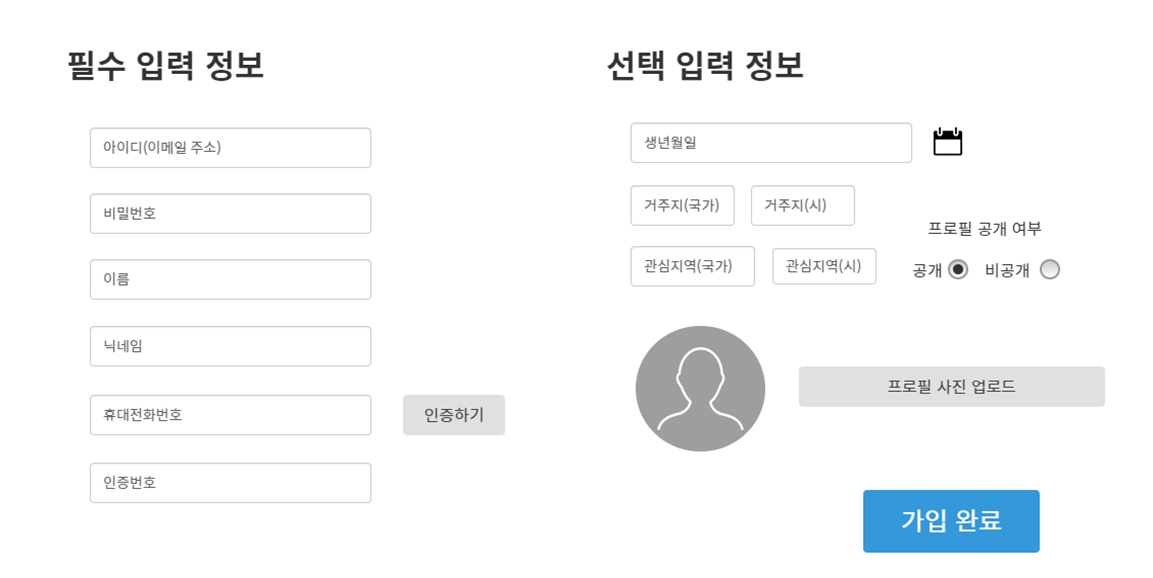
\includegraphics[width=17.00cm]{./Figure/Analysis/Display/addusert.png}} \\

    % \multicolumn{4}{|l|}{\hspace{6pt}{소셜회원 가입시}} \\ 
    \multicolumn{4}{|c|}{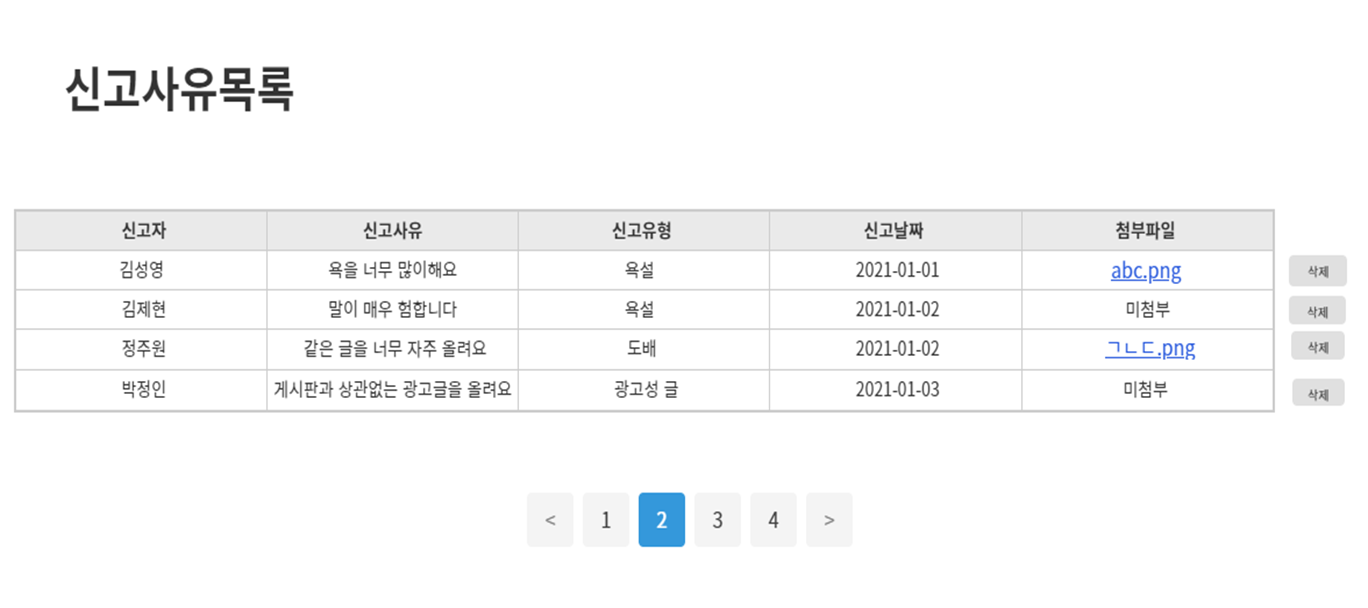
\includegraphics[width=17.00cm]{./Figure/Analysis/Display/blacklistList2.png}} \\

    \hline
\end{longtable}

\textbf{2. 데이터 구성 항목}

\begin{longtable}
    {
        |>{\centering\hspace{0pt}}m{0.150\linewidth}
        |>{\centering\hspace{0pt}}m{0.180\linewidth}
        |>{\centering\hspace{0pt}}m{0.060\linewidth}
        |>{\centering\hspace{0pt}}m{0.110\linewidth}
        |>{\hspace{0pt}}m{0.150\linewidth}
        |>{\arraybackslash\hspace{0pt}}m{0.190\linewidth}|
    } 
    \hline
    신고자 & name & Y & Y & 신고자 이름 출력 &  \\ 
    \hline
    신고사유 & reason & Y & Y & 신고사유 출력 &  \\ 
    \hline
    신고유형 & reportType & Y & Y & 신고유형 출력 &  \\ 
    \hline
    신고날짜 & reportDate & Y & Y & 신고날짜 출력 &  \\ 
    \hline
    신고자료 & proof & Y & Y & 신고자료 링크 형식으로 출력 & 링크 클릭시 사진파일 출력 \\
    \hline
\end{longtable}

\textbf{3. 처리 로직}

\arrayrulecolor{black}
\begin{longtable}
    {
        |>{\hspace{0pt}}m{0.145\linewidth}
        |>{\hspace{0pt}}m{0.140\linewidth}
        |>{\hspace{0pt}}m{0.300\linewidth}
        |>{\hspace{0pt}}m{0.140\linewidth}
        |>{\hspace{0pt}}m{0.140\linewidth}|} 
    \hline
    \rowcolor{maize} 
    \multicolumn{1}{
        |>{\centering\hspace{0pt}}m{0.145\linewidth}|}{{\cellcolor{maize}}} 
        & \multicolumn{1}{>{\centering\hspace{0pt}}m{0.140\linewidth}|}{입력값/파라미터} 
        & \multicolumn{1}{>{\centering\hspace{0pt}}m{0.300\linewidth}|}{처리내용} 
        & \multicolumn{1}{>{\centering\hspace{0pt}}m{0.140\linewidth}|}{출력/처리결과} 
        & \multicolumn{1}{>{\centering\arraybackslash\hspace{0pt}}m{0.140\linewidth}|}{{\cellcolor{maize}}} \\* 
    \hhline{|>{\arrayrulecolor{maize}}->{\arrayrulecolor{black}}|--->{\arrayrulecolor{maize}}->{\arrayrulecolor{black}}|}
    \rowcolor{maize} 
        \multicolumn{1}{|>{\Centering\hspace{0pt}}m{0.145\linewidth}|}{\multirow{-2}{=}{\cellcolor{maize}\Centering{}이벤트명}} 
        & \multicolumn{1}{>{\Centering\hspace{0pt}}m{0.140\linewidth}|}{시작 JSP} 
        & \multicolumn{1}{>{\Centering\hspace{0pt}}m{0.300\linewidth}|}{프리젠테이션 레이어 설계} 
        & \multicolumn{1}{>{\Centering\hspace{0pt}}m{0.140\linewidth}|}{출력 JSP} 
        & \multicolumn{1}{>{\Centering\hspace{0pt}}m{0.140\linewidth}|}{\multirow{-2}{=}{\cellcolor{maize}\Centering{}비고}} \endhead
    \hline
    \multirow{4}{=}{Client 요청시(onLoad()시)} &  & \multirow{2}{=}{} &  & \multirow{5}{=}{관리자권한으로만 접속가능한 페이지} \\* 
     \arrayrulecolor[rgb]{0.8,0.8,0.8}\cline{2-2}\arrayrulecolor[rgb]{0.8,0.8,0.8}\cline{4-4}
     &  &  &  &  \\* 
    \arrayrulecolor{black}\cline{2-4}
     & \multicolumn{1}{>{\hspace{0pt}}m{0.140\linewidth}|}{getBlacklist.jsp} & \multicolumn{1}{>{\hspace{0pt}}m{0.300\linewidth}|}{Path : /user/getReportList : GET} & getBlacklist.jsp &  \\* 
     \arrayrulecolor[rgb]{0.8,0.8,0.8}\cline{2-2}\arrayrulecolor{black}\cline{3-3}\arrayrulecolor[rgb]{0.8,0.8,0.8}\cline{4-4}\arrayrulecolor{black}
     &  & \multicolumn{1}{>{\hspace{0pt}}m{0.300\linewidth}|}{Controller : com.teulda.web.user.UserCont
     roller.getReportlist()} &  &  \\* 
    \arrayrulecolor{black}\hline

    \multirow{4}{=}{삭제.onClick()} & 이메일 & \multirow{2}{=}{신고내역 삭제 및 신고횟수 하락} &  &  \\* 
     \arrayrulecolor[rgb]{0.8,0.8,0.8}\cline{2-2}\arrayrulecolor[rgb]{0.8,0.8,0.8}\cline{4-4}
     &  &  &  &  \\* 
    \arrayrulecolor{black}\cline{2-5}
     & \multicolumn{1}{>{\hspace{0pt}}m{0.140\linewidth}|}{getBlacklist.jsp} & \multicolumn{1}{>{\hspace{0pt}}m{0.300\linewidth}|}{Path : /user/getReportList : GET} & getBlacklist.jsp &  \\* 
     \arrayrulecolor[rgb]{0.8,0.8,0.8}\cline{2-2}\arrayrulecolor{black}\cline{3-3}\arrayrulecolor[rgb]{0.8,0.8,0.8}\cline{4-4}\arrayrulecolor{black}
     &  & Controller : com.teulda.web.user.UserCont
     roller.getReportlist() &  &  \\ 
    \arrayrulecolor{black}\hline

    \multirow{4}{=}{확인.onClick()} & 이메일 & \multirow{2}{=}{수정내역을 갱신하고 블랙리스트 목록UI 로 Navigation} &  & \multirow{4.5}{=}{신고내역 삭제로 인해 해당 계정의 신고횟수가 10미만이 되면 자동으로 블랙리스트에서 제외} \\* 
     \arrayrulecolor[rgb]{0.8,0.8,0.8}\cline{2-2}\arrayrulecolor[rgb]{0.8,0.8,0.8}\cline{4-4}
     &  &  &  &  \\* 
    \arrayrulecolor{black}\cline{2-4}
     & \multicolumn{1}{>{\hspace{0pt}}m{0.140\linewidth}|}{getBlacklist.jsp} & \multicolumn{1}{>{\hspace{0pt}}m{0.300\linewidth}|}{Path : /user/getReportList : GET} & getBlacklist.jsp	 &  \\* 
     \arrayrulecolor[rgb]{0.8,0.8,0.8}\cline{2-2}\arrayrulecolor{black}\cline{3-3}\arrayrulecolor[rgb]{0.8,0.8,0.8}\cline{4-4}\arrayrulecolor{black}
     &  & Controller : com.teulda.web.user.UserCont
     roller.getReportlist() &  &  \\ 
    \arrayrulecolor{black}\hline
\end{longtable}
\newpage

\renewcommand{\arraystretch}{1.0}
\normalsize
\newpage